\documentclass[final]{report}

    \usepackage{ifdraft}
    \usepackage[obeyFinal]{todonotes}

    \usepackage{titlesec}
    \setcounter{secnumdepth}{3}

    \usepackage{mathrsfs}
    \usepackage{amsfonts}
    \usepackage{amssymb}
    \usepackage{dsfont}
	\usepackage{amsmath}
    \usepackage{mathtools}
    % these next 1 packages are temp \usepackage{relsize}

    \usepackage{algorithm}
    \usepackage{algpseudocode}

    \usepackage{graphicx}
		\graphicspath{{res/img/}}
	\usepackage{import}

	\usepackage{booktabs}

    \usepackage[citestyle=numeric,bibstyle=numeric]{biblatex}
        \addbibresource{bib/cdpr.bib}
        \addbibresource{bib/path_planning.bib}
        \addbibresource{bib/trajectory_generation.bib}
        \addbibresource{bib/math.bib}
		\nocite{*}

    \usepackage{parskip}


	\usepackage[hidelinks]{hyperref}
    \usepackage[all]{hypcap}

	% This should be used for full thesis:
    %\usepackage[section=section, acronyms]{glossaries}
	% This should be used for literature study report:
    \usepackage[section=subsection, acronyms]{glossaries}
        \makenoidxglossaries{}
        % Dependencies:
%	*	mathrsfs	- for mathscr font
%	*	amsfonts	- for mathfrak and mathbb (upper case) letters
%	*	amssym		- for backepsilon
%	*	dsfont		- for mathds
\newglossary*{notation}{Notation}

% ==============================================================================
% Relation Operator
% ==============================================================================
	\newcommand{\relop}{\ensuremath{\bowtie}}
	\newglossaryentry{not:relop}
	{%
		name=\ensuremath{\relop},
		description=an operator in the set \ensuremath{\{<, \leq, =, \geq, >\}},
		type=notation
	}
	\glsadd{not:relop}

% ==============================================================================
% Code
% ==============================================================================
	\newcommand{\code}[1]{\ensuremath{\texttt{#1}}}
	\newglossaryentry{not:code}
	{%
		name=\code{m},
		description=a coding function or variable,
		type=notation
	}
	\glsadd{not:code}

% ==============================================================================
% Continuity Degree
% ==============================================================================
	\newcommand{\contdeg}[1]{\ensuremath{\gls{not:contdeg}^{#1}}}
	\newglossaryentry{not:contdeg}
	{%
		name=\ensuremath{C},
		description=Degree of differentiablity
		type=notation
	}
	\glsadd{not:contdeg}
% ==============================================================================
% Geometric Continuity Degree
% ==============================================================================
	\newcommand{\contdeggeom}[1]{\ensuremath{\gls{not:contdeggeom}^{#1}}}
	\newglossaryentry{not:contdeggeom}
	{%
		name=\ensuremath{G},
		description=Geometric degree of differentiablity
		type=notation
	}
	\glsadd{not:contdeggeom}
% ==============================================================================
% differential
% ==============================================================================
	%TODO this operator is not in the nomenclature
	\newcommand{\der}{\ensuremath{\mathrm{d}}}

% ==============================================================================
% Scalar
% ==============================================================================
	\newglossaryentry{not:scalar}
	{%
		name=\ensuremath{m},
		description=a scalar,
		type=notation
	}
	\glsadd{not:scalar}

% ==============================================================================
% Vector
% ==============================================================================
	\renewcommand{\vec}[1]{\ensuremath{\boldsymbol{#1}}}
	\newglossaryentry{not:vec}
	{%
		name=\vec{m}\ifdraft{: \textbackslash{} vec}{},
		description=a vector,
		type=notation
	}
	\glsadd{not:vec}

% ==============================================================================
% Projection
% ==============================================================================
	\newcommand{\project}[2]{\ensuremath{{}^{#2}\!{#1}}}
	\newglossaryentry{not:project}
	{%
		name=\project{\vec{m}}{n}\ifdraft{: \textbackslash{} project\{to\}}{},,
		description=projection of vector \vec{m} in frame $n$,
		type=notation
	}
	\glsadd{not:project}

% ==============================================================================
% Skew Matrix
% ==============================================================================
	\newcommand{\skewmat}[1]{\ensuremath{\widehat{#1}}}
	%\newcommand{\skewmat}[1]{\ensuremath{\left[{#1}\right]_{\mathrm{X}}}}
	\newglossaryentry{not:skewmat}
	{%
		name=\skewmat{\vec{m}}\ifdraft{: \textbackslash{} skew}{},
		description=the skew matrix associated with the vector \vec{m},
		type=notation
	}
	\glsadd{not:skewmat}

% ==============================================================================
% Matrix
% ==============================================================================
	\newcommand{\mat}[1]{\ensuremath{\boldsymbol{\mathrm{#1}}}}
	\newglossaryentry{not:mat}
	{%
		name=\mat{M}\ifdraft{: \textbackslash{} mat}{},
		description=a matrix,
		type=notation
	}
	\glsadd{not:mat}

% ==============================================================================
% Pseudo Inverse
% ==============================================================================
	\newcommand{\pseudoinv}[1]{\ensuremath{{#1}^{+}}}
	\newglossaryentry{not:pseudoinv}
	{%
		name=\pseudoinv{\mat{M}}\ifdraft{: \textbackslash{} pseudoinv}{},
		description=the pseudo inverse of matrix \mat{M},
		type=notation
	}
	\glsadd{not:pseudoinv}

% ==============================================================================
% Vector Space
% ==============================================================================
	\newcommand{\vecspace}[1]{\ensuremath{\mathscr{#1}}}
	\newglossaryentry{not:vecspace}
	{%
		name=\vecspace{M}\ifdraft{: \textbackslash{} vecspace}{},
		description=a vector space,
		type=notation
	}
	\glsadd{not:vecspace}

% ==============================================================================
% Vector Norm
% ==============================================================================
	\newcommand{\norm}[1]{\ensuremath{\left|\left|#1\right|\right|}}
	\newglossaryentry{not:norm}
	{%
		name=\norm{\vec{m}}\ifdraft{: \textbackslash{} norm}{},
		description=the norm of vector $\vec{m}$,
		type=notation
	}
	\glsadd{not:norm}

% ==============================================================================
% Set
% ==============================================================================
	\newcommand{\set}[1]{\ensuremath{\mathcal{#1}}}
	\newglossaryentry{not:set}
	{%
		name=\set{M}\ifdraft{: \textbackslash{} set}{},
		description=a set,
		type=notation
	}
	\glsadd{not:set}

% ==============================================================================
% Set Cardinality
% ==============================================================================
	\newcommand{\cardinality}[1]{\ensuremath{\left|#1\right|}}
	\newglossaryentry{not:cardinality}
	{%
		name=\cardinality{M}\ifdraft{: \textbackslash{} cardinality}{},
		description=the number of elements in set $M$,
		type=notation
	}
	\glsadd{not:cardinality}

% ==============================================================================
% Function
% ==============================================================================
	\newcommand{\func}[1]{\ensuremath{\mathrm{#1}}}
	\newglossaryentry{not:func}
	{%
		name=\func{m}\ifdraft{: \textbackslash{} func}{},
		description=a function,
		type=notation
	}
	\glsadd{not:func}

% ==============================================================================
% Vector Function
% ==============================================================================
	\newcommand{\vecfunc}[1]{\ensuremath{\boldsymbol{\mathrm{#1}}}}
	\newglossaryentry{not:vecfunc}
	{%
		name=\vecfunc{m}\ifdraft{: \textbackslash{} vecfunc}{},
		description=a vector function,
		type=notation
	}
	\glsadd{not:vecfunc}

% ==============================================================================
% Estimate
% ==============================================================================
	\newcommand{\estimate}[1]{\ensuremath{\widetilde{#1}}}
	\newglossaryentry{not:estimate}
	{%
		name=\estimate{m}\ifdraft{: \textbackslash{} estimate}{},
		description=an estimate of the quantity $m$,
		type=notation
	}
	\glsadd{not:estimate}

% ==============================================================================
% Approximation
% ==============================================================================
	\newcommand{\approximation}[1]{\ensuremath{\widetilde{#1}}}
	\newglossaryentry{not:approx}
	{%
		name=\approximation{m}\ifdraft{: \textbackslash{} approx}{},
		description=an approx of the quantity $m$,
		type=notation
	}
	\glsadd{not:approx}

% ==============================================================================
% nth Time Derivative
% ==============================================================================
	\newcommand{\tdern}[2]{\ensuremath{{#1}^{(#2)}}}
	\newglossaryentry{not:tdern}
	{%
		name=\tdern{m}{n}\ifdraft{: \textbackslash{} tdern}{},
		description=the nth time derivative of quantity $m$,
		type=notation
	}
	\glsadd{not:tdern}

% ==============================================================================
% Desired Value
% ==============================================================================
	\newcommand{\desired}[1]{\ensuremath{{#1}^{*}}}
	\newglossaryentry{not:desired}
	{%
		name=\desired{m}\ifdraft{: \textbackslash{} desired}{},
		description=the desired value of $m$,
		type=notation
	}
	\glsadd{not:desired}

% ==============================================================================
% Line
% ==============================================================================
	\newcommand{\vecline}[2]{\ensuremath{\overline{#1#2}}}
	\newglossaryentry{not:line}
	{%
		name=\ensuremath{\vecline{\vec{m_1}}{\vec{m_2}}}\ifdraft{: \textbackslash{} line}{},
		description=a line connecting points $m_1$ and $m_2$,
		type=notation
	}
	\glsadd{not:line}

% ==============================================================================
% Such That
% ==============================================================================
	\newglossaryentry{not:suchthat}
	{%
		name={\ensuremath{\backepsilon}},
		description=such that,
		type=notation
	}
	\newcommand{\suchthat}{\gls{not:suchthat}}

% ==============================================================================
% Floor and Ceiling
% ==============================================================================
	\DeclarePairedDelimiter{\ceil}{\lceil}{\rceil}
	\DeclarePairedDelimiter{\floor}{\lfloor}{\rfloor}

        % Dependencies:
% 	mathabx: earth symbol
\newglossary*{symbol}{Symbols}
% ==============================================================================
% Identity Matrix
% ==============================================================================
	\newglossaryentry{sym:id}
	{%
		name=\ensuremath{\mathds{1}},
		sort=1,
		description=Identity matrix,
		type=symbol
	}
	\newcommand{\id}{\gls{sym:id}}

% ==============================================================================
% Special Orthonormal Group
% ==============================================================================
	\newglossaryentry{sym:specialOrthonormalGroup}
	{%
		name=\ensuremath{\mathrm{SO}},
		sort=se,
		description=special orthonormal group,
		type=symbol
	}
	\newcommand{\specialOrthonormalGroupbare}{\gls{sym:specialOrthonormalGroup}}
	\newcommand{\specialOrthonormalGroup}[1]{\ensuremath{\specialOrthonormalGroupbare_{#1}}}

% ==============================================================================
% Special Euclidean Group
% ==============================================================================
	\newglossaryentry{sym:specialEuclideanGroup}
	{%
		name=\ensuremath{\mathrm{SE}},
		sort=se,
		description=special euclidean group,
		type=symbol
	}
	\newcommand{\specialEuclideanGroupbare}{\gls{sym:specialEuclideanGroup}}
	\newcommand{\specialEuclideanGroup}[1]{\ensuremath{\specialEuclideanGroupbare_{#1}}}

% ==============================================================================
% Zero Vector
% ==============================================================================
	\newglossaryentry{sym:zerovec}
	{%
		name=\ensuremath{\vec{0}},
		sort=0,
		description=vector of zeros,
		type=symbol
	}
	\newcommand{\zerovec}{\gls{sym:zerovec}}

% ==============================================================================
% ==============================================================================
% ==============================================================================
% CDPR
% ==============================================================================
% ==============================================================================
% ==============================================================================

% ==============================================================================
% Angular Velocity
% ==============================================================================
	\newglossaryentry{sym:avel}
	{%
		name=\ensuremath{\vec{\omega}},
		sort=o,
		description=angular velocity,
		type=symbol
	}
	\newcommand{\avel}{\gls{sym:avel}}

% ==============================================================================
% Mass Matrix
% ==============================================================================
	\newglossaryentry{sym:transformationmat}
	{%
		name=\ensuremath{\mat{T}},
		sort=t,
		description=transformation matrix,
		type=symbol
	}
	\newcommand{\transformationmat}{\gls{sym:transformationmat}}

% ==============================================================================
% Centripetal and Coriolis Vector
% ==============================================================================
	\newglossaryentry{sym:centripitalCoriolisVec}
	{%
		name=\ensuremath{\vec{g}^c},
		sort=gc,
		description=generalised centripetal and coriolis vector,
		type=symbol
	}
	\newcommand{\centripitalCoriolisVec}{\gls{sym:centripitalCoriolisVec}}

% ==============================================================================
% Inertia Matrix
% ==============================================================================
	\newglossaryentry{sym:inertiamat}
	{%
		name=\ensuremath{\mat{I}},
			sort=i,
			description=inertia matrix,
			type=symbol
		}
		\newcommand{\inertiamat}{\gls{sym:inertiamat}}
% ==============================================================================
% Mass Matrix
% ==============================================================================
	\newglossaryentry{sym:massmat}
	{%
		name=\ensuremath{\mat{M}},
		sort=m,
		description=mass matrix,
		type=symbol
	}
	\newcommand{\massmat}{\gls{sym:massmat}}

% ==============================================================================
% Mass
% ==============================================================================
	\newglossaryentry{sym:mass}
	{%
		name=\ensuremath{m},
		sort=m,
		description=mass,
		type=symbol
	}
	\newcommand{\mass}{\gls{sym:mass}}

% ==============================================================================
% Damping Matrix
% ==============================================================================
	\newglossaryentry{sym:dampingmat}
	{%
		name=\ensuremath{\mat{D}},
		sort=d,
		description=damping matrix,
		type=symbol
	}
	\newcommand{\dampingmat}{\gls{sym:dampingmat}}

% ==============================================================================
% Workspace
% ==============================================================================
	\newglossaryentry{sym:workspace}
	{%
		name=\ensuremath{\mathcal{W}},
		sort=w,
		description=workspace of robot,
		type=symbol
	}
	\newcommand{\workspace}{\gls{sym:workspace}}

% ==============================================================================
% Loop Closure Constraints
% ==============================================================================
	\newglossaryentry{sym:loopclosureconstraints}
	{%
		name=\ensuremath{\vec{\nu}},
		sort=n,
		description=loop closure constraints,
		type=symbol
	}
	\newcommand{\loopclosureconstraints}{\gls{sym:loopclosureconstraints}}

% ==============================================================================
% Jacobian
% ==============================================================================
	\newglossaryentry{sym:jac}
	{%
		name=\ensuremath{\mat{J}},
		sort=j,
		description=Jacobian,
		type=symbol
	}
	\newcommand{\jac}{\gls{sym:jac}}

% ==============================================================================
% Geometric Jacobian
% ==============================================================================
	\newglossaryentry{sym:geometricjac}
	{%
		%TODO this should somehow use \geometricmodel directly
		name=\ensuremath{\mat{J}_{\func{g}}},
		sort=jg,
		description=Geometric Jacobian,
		type=symbol
	}
	\newcommand{\geometricjac}{\gls{sym:geometricjac}}

% ==============================================================================
% Inverse Geometric Jacobian
% ==============================================================================
	\newglossaryentry{sym:invgeometricjac}
	{%
		%TODO this should somehow use \invgeometricmodel directly
		name=\ensuremath{\mat{J}_{\func{g}^{-1}}},
		sort=jg,
		description=Inverse Geometric Jacobian,
		type=symbol
	}
	\newcommand{\invgeometricjac}{\gls{sym:invgeometricjac}}

% ==============================================================================
% Proximal Anchor
% ==============================================================================
	\newglossaryentry{sym:proximalanchor}
	{%
		name=\ensuremath{\vec{a}},
		sort=a,
		description=proximal anchor,
		type=symbol
	}
	\newcommand{\proximalanchor}{\gls{sym:proximalanchor}}

% ==============================================================================
% Distal Anchor
% ==============================================================================
	\newglossaryentry{sym:distalanchor}
	{%
		name=\ensuremath{\vec{b}},
		sort=a,
		description=distal anchor,
		type=symbol
	}
	\newcommand{\distalanchor}{\gls{sym:distalanchor}}

% ==============================================================================
% Cable Vector
% ==============================================================================
	\newglossaryentry{sym:cablevec}
	{%
		name=\ensuremath{\vec{l}},
		sort=l,
		description=cable vector,
		type=symbol
	}
	\newcommand{\cablevec}{\gls{sym:cablevec}}

% ==============================================================================
% Cable Unit Vector
% ==============================================================================
	\newglossaryentry{sym:cableuvec}
	{%
		name=\ensuremath{\vec{u}},
		sort=u,
		description=cable unit vector,
		type=symbol
	}
	\newcommand{\cableuvec}{\gls{sym:cableuvec}}

% ==============================================================================
% Cable Length
% ==============================================================================
	\newglossaryentry{sym:cablelength}
	{%
		name=\ensuremath{l},
		sort=l,
		description=the lengths of a cable,
		type=symbol
	}
	\newcommand{\cablelength}{\gls{sym:cablelength}}

% ==============================================================================
% Cable Lengths
% ==============================================================================
	\newglossaryentry{sym:cablelengths}
	{%
		name=\ensuremath{\mat{l}},
		sort=l,
		description=the lengths of the cables \ensuremath{\mat{l} = {\left[\begin{matrix}l_1 & \cdots & l_m \end{matrix}\right]}^T},
		type=symbol
	}
	\newcommand{\cablelengths}{\gls{sym:cablelengths}}

% ==============================================================================
% Translation Vector
% ==============================================================================
	\newglossaryentry{sym:transvec}
	{%
		name=\ensuremath{\vec{t}},
		sort=t,
		description=translation vector,
		type=symbol
	}
	\newcommand{\transvec}{\gls{sym:transvec}}

% ==============================================================================
% Rotation Matrix
% ==============================================================================
	\newglossaryentry{sym:rotmat}
	{%
		name=\ensuremath{\mat{R}},
		sort=r,
		description=rotaion matrix,
		type=symbol
	}
	\newcommand{\rotmatbare}{\gls{sym:rotmat}}
	\newcommand{\rotmat}[2]{{\project{\rotmatbare}{#1}}_{#2}}

% ==============================================================================
% Set of Rotation Matrices
% ==============================================================================
	\newglossaryentry{sym:setofrotationmatrices}
	{%
		name=\ensuremath{\set{R}},
		sort=r,
		description=set of rotaion matrices,
		type=symbol
}
\newcommand{\setofrotationmatrices}{\gls{sym:setofrotationmatrices}}

% ==============================================================================
% Structure Matrix
% ==============================================================================
	\newglossaryentry{sym:strucmat}
	{%
		name=\ensuremath{{\mat{A}^T}},
		sort=a,
		description=structure matrix,
		type=symbol
	}
	\newcommand{\strucmat}{\gls{sym:strucmat}}

% ==============================================================================
% Set of Solutions to Structure Equation
% ==============================================================================
	\newglossaryentry{sym:setsolstruceq}
	{%
		name=\ensuremath{\set{S}},
		sort=s,
		description=set of solutions to the structure equation,
		type=symbol
	}
	\newcommand{\setsolstruceq}{\gls{sym:setsolstruceq}}

% ==============================================================================
% Set of Feasible Force Distributions
% ==============================================================================
	\newglossaryentry{sym:setoffeasibleforces}
	{%
		name=\ensuremath{\set{T}},
		sort=t,
		description=set of feasible force distributions in the cables,
		type=symbol
	}
	\newcommand{\setoffeasibleforces}{\gls{sym:setoffeasibleforces}}

% ==============================================================================
% End Effector Pose
% ==============================================================================
	\newglossaryentry{sym:pose}
	{%
		name=\ensuremath{\vec{y}},
		sort=y,
		description=pose of the end-effector \ensuremath{\vec{y} = (\transvec, \rotmatbare)},
		type=symbol
	}
	\newcommand{\pose}{\gls{sym:pose}}

% ==============================================================================
% Set of End Effector Poses
% ==============================================================================
	\newglossaryentry{sym:setofposes}
	{%
		name=\ensuremath{\set{Y}},
		sort=y,
		description=set of poses of the end-effector,
		type=symbol
	}
	\newcommand{\setofposes}{\gls{sym:setofposes}}

% ==============================================================================
% Cartesian Frame
% ==============================================================================
	\newglossaryentry{sym:frame}
	{%
		name=\ensuremath{\mathscr{F}},
		sort=f,
		description=frame,
		type=symbol
	}
	\newcommand{\framesym}{\gls{sym:frame}}

% ==============================================================================
% Platform
% ==============================================================================
	%TODO this should be in subscripts
	\newglossaryentry{sym:platform}
	{%
		name=\ensuremath{\mathscr{P}},
		sort=p,
		description=platform,
		type=symbol
	}
	\newcommand{\platform}{\gls{sym:platform}}
	\newcommand{\platformframe}{\framesym_{\platform}}
	\newcommand{\worldframe}{\framesym_{0}} %TODO this should have its own thing, also put Earth

% ==============================================================================
% Robot DOF
% ==============================================================================
	\newglossaryentry{sym:robotdof}
	{%
		name=\ensuremath{n},
		sort=n,
		description=robot degrees of freedom,
		type=symbol
	}
	\newcommand{\robotdof}{\gls{sym:robotdof}}

% ==============================================================================
% Number of Cables
% ==============================================================================
	\newglossaryentry{sym:numcables}
	{%
		name=\ensuremath{m},
		sort=m,
		description=number of cables,
		type=symbol
	}
	\newcommand{\numcables}{\gls{sym:numcables}}

% ==============================================================================
% Degree of Redundancy
% ==============================================================================
	\newglossaryentry{sym:degofredundancy}
	{%
		name=\ensuremath{r},
		sort=r,
		description=degree of redunancy,
		type=symbol
	}
	\newcommand{\degofredundancy}{\gls{sym:degofredundancy}}

% ==============================================================================
% Cell
% ==============================================================================
	\newglossaryentry{sym:cell}
	{%
		name=\ensuremath{\set{C}},
		sort=c,
		description=cell,
		type=symbol
	}
	\newcommand{\cell}{\gls{sym:cell}}

% ==============================================================================
% Sample
% ==============================================================================
	\newglossaryentry{sym:sample}
	{%
		name=\ensuremath{\sigma},
		sort=s,
		description=sample,
		type=symbol
	}
	\newcommand{\sample}{\gls{sym:sample}}

% ==============================================================================
% Distance
% ==============================================================================
	\newglossaryentry{sym:distance}
	{%
		name=\ensuremath{d},
		sort=h,
		description=distance,
		type=symbol
	}
	\newcommand{\distance}{\gls{sym:distance}}

% ==============================================================================
% Quaternion
% ==============================================================================
	\newglossaryentry{sym:quaternion}
	{%
		name=\ensuremath{\vec{h}},
		sort=h,
		description=quaternion,
		type=symbol
	}
	\newcommand{\quaternion}{\gls{sym:quaternion}}

% ==============================================================================
% Quaternion Imaginary part
% ==============================================================================
	\newglossaryentry{sym:quaternionimg}
	{%
		name=\ensuremath{\vec{h}_{\mathrm{Im}}}, %TODO should be in subscripts
		sort=h,
		description=imaginary vector part of a quaterion,
		type=symbol
	}
	\newcommand{\quaternionimg}{\gls{sym:quaternionimg}}

% ==============================================================================
% Quaternion Real Part
% ==============================================================================
	\newglossaryentry{sym:quaternionre}
	{%
		name=\ensuremath{h_{\mathrm{Re}}}, %TODO should be in subscripts
		sort=h,
		description=Scalar real part of a quaternion,
		type=symbol
	}
	\newcommand{\quaternionre}{\gls{sym:quaternionre}}

% ==============================================================================
% Quaternion Derivative to Angular Velocity Transformation
% ==============================================================================
	\newglossaryentry{sym:quaternionToAvelTrans}
	{%
		name=\ensuremath{\mat{P}}, %TODO should be in subscripts
		sort=p,
		description=transformation matrix relating quaternion derivative to angular velocity,
		type=symbol
	}
	\newcommand{\quaternionToAvelTrans}{\gls{sym:quaternionToAvelTrans}}

% ==============================================================================
% Queue
% ==============================================================================
	\newglossaryentry{sym:queue}
	{%
		name=\ensuremath{\code{q}},
		sort=q,
		description=queue,
		type=symbol
	}
	\newcommand{\queue}{\gls{sym:queue}}

% ==============================================================================
% Force Magnitude
% ==============================================================================
	\newglossaryentry{sym:forcemag}
	{%
		name=\ensuremath{f},
		sort=f,
		description=magnitude of force,
		type=symbol
	}
	\newcommand{\forcemag}{\gls{sym:forcemag}}

% ==============================================================================
% Force Magnitude Vector
% ==============================================================================
	\newglossaryentry{sym:forcemagvec}
	{%
		name=\ensuremath{\mat{f}},
		sort=f,
		description=vector of force magnitudes,
		type=symbol
	}
	\newcommand{\forcemagvec}{\gls{sym:forcemagvec}}

% ==============================================================================
% Force
% ==============================================================================
	\newglossaryentry{sym:force}
	{%
		name=\ensuremath{\vec{f}},
		sort=f,
		description=force,
		type=symbol
	}
	\newcommand{\force}{\gls{sym:force}}

% ==============================================================================
% Torque
% ==============================================================================
	\newglossaryentry{sym:torque}
	{%
		name=\ensuremath{\vec{\tau}},
		sort=t,
		description=torque,
		type=symbol
	}
	\newcommand{\torque}{\gls{sym:torque}}

% ==============================================================================
% Twist
% ==============================================================================
	\newglossaryentry{sym:twist}
	{%
		name=\ensuremath{\vec{\xi}},
		sort=t,
		description=twist,
		type=symbol
	}
	\newcommand{\twist}{\gls{sym:twist}}

% ==============================================================================
% Wrench
% ==============================================================================
	\newglossaryentry{sym:wrench}
	{%
		name=\ensuremath{\vec{\zeta}},
		sort=t,
		description=wrench,
		type=symbol
	}
	\newcommand{\wrench}{\gls{sym:wrench}}

% ==============================================================================
% Set of Wrenches
% ==============================================================================
	\newglossaryentry{sym:setofwrenches}
	{%
		name=\ensuremath{\set{Q}},
		sort=q,
		description=set of wrenches,
		type=symbol
	}
	\newcommand{\setofwrenches}{\gls{sym:setofwrenches}}

% ==============================================================================
% Gain
% ==============================================================================
	\newglossaryentry{sym:gain}
	{%
		name={\ensuremath{\lambda}},
		sort=l,
		description=A tunable gain,
		type=symbol
	}
	\newcommand{\gain}{\gls{sym:gain}}

% ==============================================================================
% Point
% ==============================================================================
	\newglossaryentry{sym:point}
	{%
		name={\ensuremath{\vec{p}}},
		sort=p,
		description=A point in space,
		type=symbol
	}
	\newcommand{\point}{\gls{sym:point}}

% ==============================================================================
% Set of Points
% ==============================================================================
	\newglossaryentry{sym:setofpoints}
	{%
		name={\ensuremath{\set{P}}},
		sort=p,
		description=A set of points in space,
		type=symbol
	}
	\newcommand{\setofpoints}{\gls{sym:setofpoints}}

% ==============================================================================
% Trajectory
% ==============================================================================
	\newglossaryentry{sym:traj}
	{%
		name={\ensuremath{\vec{s}}},
		sort=s,
		description=A trajectory in space,
		type=symbol
	}
	\newcommand{\traj}{\gls{sym:traj}}

% ==============================================================================
% Path
% ==============================================================================
	\newcommand{\pathsym}{\traj}


% ==============================================================================
% Time
% ==============================================================================
	\newglossaryentry{sym:time}
	{%
		name={\ensuremath{t}},
		sort=t,
		description=time,
		type=symbol
	}
	\newcommand{\timesym}{\gls{sym:time}}

% ==============================================================================
% Time Normalised
% ==============================================================================
	\newglossaryentry{sym:timenorm}
	{%
		name={\ensuremath{\tau}},
		sort=t,
		description=normalised time \ensuremath{\tau \in [0, 1]},
		type=symbol
	}
	\newcommand{\timenorm}{\gls{sym:timenorm}}

% ==============================================================================
% Set of Time Instants
% ==============================================================================
	\newglossaryentry{sym:setoftimeinstants}
	{%
		name={\ensuremath{\set{T}}},
		sort=t,
		description=A set of time instants,
		type=symbol
	}
	\newcommand{\setoftimeinstants}{\gls{sym:setoftimeinstants}}

% ==============================================================================
% Period
% ==============================================================================
	\newglossaryentry{sym:period}
	{%
		name={\ensuremath{T}},
		sort=t,
		description=period,
		type=symbol
	}
	\newcommand{\period}{\gls{sym:period}}

% ==============================================================================
% Tolerance
% ==============================================================================
	\newglossaryentry{sym:tolerance}
	{%
		name={\ensuremath{\epsilon}},
		sort=e,
		description=Tolerance,
		type=symbol
	}
	\newcommand{\tol}{\gls{sym:tolerance}}

% ==============================================================================
% Tolerance
% ==============================================================================
	\newglossaryentry{sym:threshold}
	{%
		name={\ensuremath{\delta}},
		sort=d,
		description=Threshold,
		type=symbol
	}
	\newcommand{\threshold}{\gls{sym:threshold}}

% ==============================================================================
% Geometric Model
% ==============================================================================
	\newglossaryentry{sym:geometricmodel}
	{%
		name={\ensuremath{\vecfunc{g}}},
		sort=G,
		description=Geometric Model,
		type=symbol
	}
	\newcommand{\geometricmodel}{\gls{sym:geometricmodel}}

% ==============================================================================
% Inverse Geometric Model
% ==============================================================================
	\newglossaryentry{sym:invgeometricmodel}
	{%
		name={\ensuremath{{\vecfunc{g}^{-1}}}},
		sort=G,
		description=Inverse Geometric Model,
		type=symbol
	}
	\newcommand{\invgeometricmodel}{\gls{sym:invgeometricmodel}}
% ==============================================================================
% Kinematic Model
% ==============================================================================
	\newglossaryentry{sym:kinematicmodel}
	{%
		name={\ensuremath{\vecfunc{k}}},
		sort=K,
		description=Kinematic Model,
		type=symbol
	}
	\newcommand{\kinematicmodel}{\gls{sym:kinematicmodel}}

% ==============================================================================
% Inverse Kinematic Model
% ==============================================================================
	\newglossaryentry{sym:invkinematicmodel}
	{%
		name={\ensuremath{{\vecfunc{k}^{-1}}}},
		sort=K,
		description=Inverse Kinematic Model,
		type=symbol
	}
	\newcommand{\invkinematicmodel}{\gls{sym:invkinematicmodel}}
% ==============================================================================
% Dynamic Model
% ==============================================================================
	\newglossaryentry{sym:dynamicmodel}
	{%
		name={\ensuremath{\vecfunc{d}}},
		sort=d,
		description=Dynamic Model,
		type=symbol
	}
	\newcommand{\dynamicmodel}{\gls{sym:dynamicmodel}}

% ==============================================================================
% Inverse Dynamic Model
% ==============================================================================
	\newglossaryentry{sym:invdynamicmodel}
	{%
		name={\ensuremath{{\vecfunc{d}^{-1}}}},
		sort=d,
		description=Inverse Dynamic Model,
		type=symbol
	}
	\newcommand{\invdynamicmodel}{\gls{sym:invdynamicmodel}}

% ==============================================================================
% Constraint
% ==============================================================================
	\newglossaryentry{sym:constraint}
	{%
		%name=\protect\reflectbox{\ensuremath{\mathds{C}}},
		%name=\protect\reflectbox{\ensuremath{\mat{C}}},
		name=\ensuremath{c},
		sort=c,
		description=constraint,
		type=symbol
	}
	\newcommand{\constraint}{\gls{sym:constraint}}

% ==============================================================================
% Set of Constraints
% ==============================================================================
	\newglossaryentry{sym:setofconstraints}
	{%
		%name=\protect\reflectbox{\ensuremath{\set{C}}},
		%name=\protect\reflectbox{\ensuremath{\mat{C}}},
		name=\ensuremath{\set{C}},
		sort=c,
		description=set of constraints,
		type=symbol
	}
	\newcommand{\setofconstraints}{\gls{sym:setofconstraints}}

% ==============================================================================
% Configuration
% ==============================================================================
	\newglossaryentry{sym:configuration}
	{%
		name=\ensuremath{q},
		sort=q,
		description=Configuration,
		type=symbol
	}
	\newcommand{\configuration}{\gls{sym:configuration}}

%TODO indexes
% ==============================================================================
% Index i
% ==============================================================================
	\newglossaryentry{sym:indexi}
	{%
		name=\ensuremath{i},
		sort=i,
		description=an index,
		type=symbol
	}
	\newcommand{\indexi}{\gls{sym:indexi}}
% ==============================================================================
% Index j
% ==============================================================================
	\newglossaryentry{sym:indexj}
	{%
		name=\ensuremath{j},
		sort=j,
		description=an index,
		type=symbol
	}
	\newcommand{\indexj}{\gls{sym:indexj}}

% ==============================================================================
% Index k
% ==============================================================================
	\newglossaryentry{sym:indexk}
	{%
		name=\ensuremath{k},
		sort=k,
		description=an index,
		type=symbol
	}
	\newcommand{\indexk}{\gls{sym:indexk}}

% ==============================================================================
% State
% ==============================================================================
	\newglossaryentry{sym:state}
	{%
		name=\ensuremath{\vec{x}},
		sort=x,
		description=the state  of the robot,
		type=symbol
	}
	\newcommand{\state}{\gls{sym:state}}

% ==============================================================================
% State Space
% ==============================================================================
	\newglossaryentry{sym:statespace}
	{%
		name=\ensuremath{\vecspace{X}},
		sort=x,
		description=the state space of the robot,
		type=symbol
	}
	\newcommand{\statespace}{\gls{sym:statespace}}

% ==============================================================================
% Phase Space
% ==============================================================================
	\newcommand{\phasespace}{\statespace}

% ==============================================================================
% Inverse Action
% ==============================================================================
	\newglossaryentry{sym:invaction}
	{%
		name=\ensuremath{\vec{u}^{-1}},
		sort=u,
		description=the inverse action  of the robot,
		type=symbol
	}
	\newcommand{\invaction}{\gls{sym:invaction}}
% ==============================================================================
% Action
% ==============================================================================
	\newglossaryentry{sym:action}
	{%
		name=\ensuremath{\vec{u}},
		sort=u,
		description=the action  of the robot,
		type=symbol
	}
	\newcommand{\action}{\gls{sym:action}}

% ==============================================================================
% Action Space
% ==============================================================================
	\newglossaryentry{sym:actionspace}
	{%
		name=\ensuremath{\vecspace{U}},
		sort=u,
		description=the action space of the robot,
		type=symbol
	}
	\newcommand{\actionspace}{\gls{sym:actionspace}}

% ==============================================================================
% Inverse Action Space
% ==============================================================================
	\newglossaryentry{sym:invactionspace}
	{%
		name=\ensuremath{\vecspace{U}^{-1}},
		sort=u,
		description=the inverse action space of the robot,
		type=symbol
	}
	\newcommand{\invactionspace}{\gls{sym:invactionspace}}

% ==============================================================================
% Configuration Space
% ==============================================================================
	\newglossaryentry{sym:configurationspace}
	{%
		name=\ensuremath{\vecspace{C}},
		sort=c,
		description=the configuration space of the robot,
		type=symbol
	}
	\newcommand{\configurationspace}{\gls{sym:configurationspace}}
% ==============================================================================
% World Space
% ==============================================================================
	\newglossaryentry{sym:worldspace}
	{%
		name=\ensuremath{\vecspace{W}},
		sort=w,
		description=the world inhabited by the robot,
		type=symbol
	}
	\newcommand{\world}{\gls{sym:worldspace}}

%%TODO Polynomials
% ==============================================================================
% B-Spline
% ==============================================================================
	\newglossaryentry{sym:bspline}
	{%
		name=\ensuremath{\vec{B}},
		sort=b,
		description=B-spline basis function,
		type=symbol
	}
	\newcommand{\bspline}{\gls{sym:bspline}}
% ==============================================================================
% knot
% ==============================================================================
	\newglossaryentry{sym:knot}
	{%
		name=\ensuremath{\vec{k}},
		sort=k,
		description=B-spline knot vector,
		type=symbol
	}
	\newcommand{\knot}{\gls{sym:knot}}
% ==============================================================================
% Coefficient
% ==============================================================================
	\newglossaryentry{sym:polynomial}
	{%
		name=\ensuremath{\func{p}},
		sort=p,
		description=a polynomial function,
		type=symbol
	}
	\newcommand{\polynomial}{\gls{sym:polynomial}}

% ==============================================================================
% Coefficient
% ==============================================================================
	\newglossaryentry{sym:coefficient}
	{%
		name=\ensuremath{a},
		sort=a,
		description=Polynomial Coefficient,
		type=symbol
	}
	\newcommand{\coefficient}{\gls{sym:coefficient}}

% ==============================================================================
% Coefficient
% ==============================================================================
	\newglossaryentry{sym:coefficientb}
	{%
		name=\ensuremath{b},
		sort=b,
		description=Polynomial Coefficient,
		type=symbol
	}
	\newcommand{\coefficientb}{\gls{sym:coefficientb}}

% ==============================================================================
% Polynomial Degree
% ==============================================================================
	\newglossaryentry{sym:poldeg}
	{%
		name=\ensuremath{n},
		sort=n,
		description=Polynomial Degree,
		type=symbol
	}
	\newcommand{\poldeg}{\gls{sym:poldeg}}

% ==============================================================================
% Polynomial Degree
% ==============================================================================
	\newglossaryentry{sym:relweight}
	{%
		name=\ensuremath{\mu},
		sort=m,
		description=relative weight of a factor \ensuremath{\mu \in [0, 1]},
		type=symbol
	}
	\newcommand{\relweight}{\gls{sym:relweight}}

% ==============================================================================
% Half Space Primitive
% ==============================================================================
	\newglossaryentry{sym:halfspaceprimitive}
	{%
		name=\ensuremath{\set{H}},
		sort=h,
		description=a half space primitive,
		type=symbol
	}
	\newcommand{\halfspaceprimitive}{\gls{sym:halfspaceprimitive}}

% ==============================================================================
% Transform function
% ==============================================================================
	\newglossaryentry{sym:transform}
	{%
		name=\ensuremath{\func{h}},
		sort=h,
		description=a transform function,
		type=symbol
	}
	\newcommand{\transform}{\gls{sym:transform}}

% ==============================================================================
% Robot
% ==============================================================================
	\newglossaryentry{sym:robot}
	{%
		name=\ensuremath{\set{A}},
		sort=a,
		description=a robot,
		type=symbol
	}
	\newcommand{\robot}{\gls{sym:robot}}

% ==============================================================================
% Point in Robot
% ==============================================================================
	\newglossaryentry{sym:pointinrobot}
	{%
		name=\ensuremath{\vec{a}},
		sort=a,
		description=a point in a robot,
		type=symbol
	}
	\newcommand{\pointinrobot}{\gls{sym:pointinrobot}}

% ==============================================================================
% Obstacle
% ==============================================================================
	\newglossaryentry{sym:obstacle}
	{%
		name=\ensuremath{\set{O}},
		sort=o,
		description=an obstacle,
		type=symbol
	}
	\newcommand{\obstacle}{\gls{sym:obstacle}}

% ==============================================================================
% Obstacle
% ==============================================================================
	\newglossaryentry{sym:logicalpredicate}
	{%
		name=\ensuremath{\func{\phi}},
		sort=f,
		description=an logical predicate,
		type=symbol
	}
	\newcommand{\logicalpredicate}{\gls{sym:logicalpredicate}}

% ==============================================================================
% True
% ==============================================================================
	\newglossaryentry{sym:true}
	{%
		name=\ensuremath{\top},
		sort=t,
		description=true,
		type=symbol
	}
	\newcommand{\true}{\gls{sym:true}}

% ==============================================================================
% False
% ==============================================================================
	\newglossaryentry{sym:false}
	{%
		name=\ensuremath{\bot},
		sort=t,
		description=false,
		type=symbol
	}
	\newcommand{\false}{\gls{sym:false}}

% ==============================================================================
% Swath
% ==============================================================================
	\newglossaryentry{sym:swath}
	{%
		name=\ensuremath{\set{S}},
		sort=s,
		description=the set of points reached by a topological graph,
		type=symbol
	}
	\newcommand{\swath}{\gls{sym:swath}}

% ==============================================================================
% Graph
% ==============================================================================
	\newglossaryentry{sym:topologicalgraph}
	{%
		name=\ensuremath{\set{G}},
		sort=g,
		description=topological graph,
		type=symbol
	}
	\newcommand{\topologicalgraph}{\gls{sym:topologicalgraph}}

% ==============================================================================
% Edge
% ==============================================================================
	\newglossaryentry{sym:edge}
	{%
		name=\ensuremath{\vec{e}},
		sort=e,
		description=edge of a graph,
		type=symbol
	}
	\newcommand{\edge}{\gls{sym:edge}}

% ==============================================================================
% Vertex
% ==============================================================================
	\newglossaryentry{sym:vertex}
	{%
		name=\ensuremath{\vec{v}},
		sort=e,
		description=vertex of a graph,
		type=symbol
	}
	\newcommand{\vertex}{\gls{sym:vertex}}

% ==============================================================================
% Convex Hull
% ==============================================================================
	\newglossaryentry{sym:convexhull}
	{%
		name=\ensuremath{\func{Conv}},
		sort=0,
		description=convex hull of a set,
		type=symbol
	}
	\newcommand{\convexhull}{\gls{sym:convexhull}}

% ==============================================================================
% ==============================================================================
% ==============================================================================
% CSP
% ==============================================================================
% ==============================================================================
% ==============================================================================

% ==============================================================================
% CSP function
% ==============================================================================
	\newglossaryentry{sym:cspfunc}
	{%
		name=\ensuremath{\vecfunc{\phi}},
		sort=f,
		description=CSP function,
		type=symbol
	}
	\newcommand{\cspfunc}{\gls{sym:cspfunc}}

% ==============================================================================
% Calculation Variables
% ==============================================================================
	\newglossaryentry{sym:calcvars}
	{%
		name=\ensuremath{\vec{c}},
		sort=f,
		description=calculation variables of CSP,
		type=symbol
	}
	\newcommand{\calcvars}{\gls{sym:calcvars}}

% ==============================================================================
% Verification Variables
% ==============================================================================
	\newglossaryentry{sym:vervars}
	{%
		name=\ensuremath{\vec{v}},
		sort=f,
		description=verification variables of CSP,
		type=symbol
	}
	\newcommand{\vervars}{\gls{sym:vervars}}

% ==============================================================================
% Verification Domain
% ==============================================================================
	\newglossaryentry{sym:verdomain}
	{%
		name=\ensuremath{\set{X}_{v}},
		sort=f,
		description=verification domain of CSP,
		type=symbol
	}
	\newcommand{\verdomain}{\gls{sym:verdomain}}

% ==============================================================================
% CSP Search Space
% ==============================================================================
	\newglossaryentry{sym:cspsearchspace}
	{%
		name=\ensuremath{\set{X}_{s}},
		sort=f,
		description=search space of CSP,
		type=symbol
	}
	\newcommand{\cspsearchspace}{\gls{sym:cspsearchspace}}

% ==============================================================================
% CSP Solution Set
% ==============================================================================
	\newglossaryentry{sym:cspsolutionset}
	{%
		name=\ensuremath{\set{X}_{c}},
		sort=f,
		description=solution set of CSP,
		type=symbol
	}
	\newcommand{\cspsolutionset}{\gls{sym:cspsolutionset}}

        \newacronym{dof}{dof}{Degree of Freedom}
\newacronym{cdpr}{CDPR}{Cable-Driven Parallel Robot}
\newacronym{dgm}{DGM}{Direct Geometric Model}
\newacronym{igm}{IGM}{Indirect Geometric Model}
\newacronym{dkm}{DKM}{Direct Kinematic Model}
\newacronym{ikm}{IKM}{Indirect Kineamtic Model}
\newacronym{ddm}{DDM}{Direct Dynamic Model}
\newacronym{idm}{IDM}{Inverse Dynamic Model}
\newacronym{fifo}{FIFO}{First-In-First-Out}
\newacronym{lifo}{LIFO}{Last-In-First-Out}

        \newglossary*{defs}{Glossary}

\newglossaryentry{jolt}
{%
	name=jolt,
	description=The first time derivative of acceleration (in some texts referred to as ``jerk''),
	type=defs
}

\newglossaryentry{jounce}
{%
	name=jounce,
	description=The second time derivative of acceleration,
	type=defs
}

        \newglossary*{subscript}{Subscripts}

% ==============================================================================
% Final
% ==============================================================================
	\newglossaryentry{sub:final}
	{%
		name={\ensuremath{\mathrm{F}}},
		sort=f,
		description=Final,
		type=subscript
	}
	\newcommand{\final}{\gls{sub:final}}

% ==============================================================================
% Goal
% ==============================================================================
	\newglossaryentry{sub:goal}
	{%
		name={\ensuremath{\mathrm{G}}},
		sort=g,
		description=goal,
		type=subscript
	}
	\newcommand{\goal}{\gls{sub:goal}}

% ==============================================================================
% Initial
% ==============================================================================
	\newglossaryentry{sub:initial}
	{%
		name={\ensuremath{\mathrm{I}}},
		sort=i,
		description=initial,
		type=subscript
	}
	\newcommand{\initial}{\gls{sub:initial}}

% ==============================================================================
% Obstacle Region
% ==============================================================================
	\newglossaryentry{sub:obstacleregion}
	{%
		name={\ensuremath{\mathrm{obs}}},
		sort=obs,
		description=obstacle region,
		type=subscript
	}
	\newcommand{\obstacleregion}{\gls{sub:obstacleregion}}

% ==============================================================================
% Free Region
% ==============================================================================
	\newglossaryentry{sub:freeregion}
	{%
		name={\ensuremath{\mathrm{free}}},
		sort=obs,
		description=free region,
		type=subscript
	}
	\newcommand{\freeregion}{\gls{sub:freeregion}}

		\setlength{\glslistdottedwidth}{4cm}
        \setglossarystyle{listdotted}
        \ifdraft{\glsaddall}{}

	% redefine sections for literature report only
	\let\paragraph\subsubsection%
	\let\subsubsection\subsection%
	\let\subsection\section%
	\let\section\chapter%

\begin{document}

	\ifdraft{\listoftodos{}}{}

	\def\lskip{\vspace{0.5cm}}


\begin{tabular}{p{7cm}p{8cm}}
	ÉCOLE CENTRALE DE NANTES & UNIVERSITÀ DEGLI STUDI DI GENOVA
\end{tabular}

\vspace{2cm}

\begin{center}
	\large\sc MASTER ERASMUS MUNDUS \\ 
	\normalsize{EMARO+ ``European Master in Advanced Robotics''}
\end{center}

\begin{center}
	2018 / 2019
	\lskip%

	Thesis Report
	\lskip%

	Presented by
	\lskip%

	Hendrik Scheepers de Bruin
	\lskip%

	22 July 2019
	\lskip\lskip%

	{\Large \textbf{Path Planning for Cable-Driven Parallel Robots}}

\end{center}

\vfill

\begin{center}
	Jury
\end{center}

\begin{tabular}{p{0.2\textwidth} p{0.4\textwidth} p{0.4\textwidth}}
	President:		& Olivier KERMORGANT	& Assistant Professor (LS2N) \\
	\\
	Evaluators:		& Philippe Wenger 		& Assistant Professor (LS2N) \\
	\\
	Supervisors:	& Nicolò PEDEMONTE		& Researcher (IRT Jules Verne) \\
					& Stéphane CARO			& Researcher (CNRS - LS2N) \\
	%(EMARO)  & Co-supervisor from M1 & Position, M1 institution
\end{tabular}

\lskip%

Laboratory: Laboratoire des Sciences du Numérique de Nantes LS2N

    \begin{abstract}

	Lorem in excepturi veniam sed minima voluptatem suscipit. Fugit maiores
	distinctio fuga nobis temporibus Vero quod nam dolores beatae deserunt.
	Velit placeat sit culpa qui nostrum! Voluptates aperiam nisi repellendus
	possimus quis fugiat. Illum maxime est pariatur perspiciatis mollitia porro
	Deleniti cum libero ipsa a minus Necessitatibus aut cumque facere illum eum.

	Non saepe maiores facilis blanditiis consectetur. Illo placeat consectetur
	cumque sed iusto minus Reiciendis minus maxime sint eum nihil Voluptas
	quibusdam provident necessitatibus commodi at Eos vitae perspiciatis maxime
	ab doloribus Quo amet consequuntur doloribus nulla quisquam Tempora magnam
	tenetur ex atque fuga Exercitationem perferendis eligendi fugit voluptatum
	adipisci Odit quisquam dolore deleniti impedit similique. Inventore magni
	nihil itaque labore unde? Natus culpa amet corporis laborum deserunt numquam
	Illum nihil reprehenderit fuga nam magni reiciendis. Debitis enim fugiat
	expedita earum repudiandae Voluptas nisi cumque necessitatibus laboriosam
	odit.

\end{abstract}


    \clearpage
    \pagenumbering{roman}

    \tableofcontents
    \listoffigures
    \listoftables
    \listofalgorithms{}
    \chapter*{Nomenclature}

	\todo{Notation entry is commented out}
	\todo{make subscript nomenclature}
	\printnoidxglossary[type=acronym, sort=case]
	\printnoidxglossary[type=defs,style=super4col]
	\printnoidxglossary[type=notation, sort=def]
	\printnoidxglossary[type=symbol, sort=case]
	\printnoidxglossary[type=subscript, sort=case]


    \clearpage
    \pagenumbering{arabic}
    \chapter{Introduction}%
\label{chap:introduction}

	\glsresetall

	\glspl{cdpr} are a class of robot where the end-effector is suspended and
	supported by cables. The cables are connected to spools. Through actuation
	of the spools, the end-effector's pose in space may be controlled.

	Using cables for end-effector manipulation has some benefits over
	traditional serial and parallel robots. Cables are very lightweight.
	\glspl{cdpr} therefore tend to require smaller motors and are consequently
	inexpensive as compared to similar traditional robots. Furthermore, since
	cables are flexible, \glspl{cdpr} can be designed to be easily portable and
	reconfigurable. Due to their inexpensive and lightweight topology,
	\glspl{cdpr} can be made to cover very vast workspaces and are able to
	obtain very high velocities and accelerations.

	The added flexibility of this class of robot comes at a cost, however. When
	compared to traditional parallel robots, \glspl{cdpr} have the added
	constraint that all cables need to be in tension. That is, it is not
	possible to have a link push the end-effector as is the case with
	traditional robots. Furthermore, \glspl{cdpr} exhibit further new
	challenges, such as cable sagging and vibration.

	\glspl{cdpr} have seen few practical applications to date. However, due to
	their potential, they have started attracting more interest in the research
	community.

	A common problem in robotics is the generation of trajectories.  When
	generating non-trivial trajectories for \glspl{cdpr}, care must be taken to
	avoid any obstacles in the workspace. This is complicated by the fact that
	the cables which support the robot can span large sections of the workspace.
	Rotational trajectories can also cause cable-cable or cable-platform
	collisions. The current thesis report documents an approach to generating
	collision-free trajectories in $\specialEuclideanGroup{3}$ in the presence
	of obstacles.


    \chapter{Literature Study}%
\label{chap:literature_study}

	The literature study for the present report has three main sections.
	Section~\ref{sec:trajectory_generation} reviews techniques for generating
	trajectories that meet certain criteria. Section~\ref{sec:path_planning}
	gives an overview of path planning methodologies. Finally,
	Section~\ref{sec:modelling_of_cable_driven_parallel_robots} gives an
	overview of the important aspects in modelling \glspl{cdpr}.

	\section{Trajectory Generation}%
\label{sec:trajectory_generation}

	The problem of trajectory generation can be categorised into one-dimensional
	and multi-dimensional trajectories. A schematic overview is shown in
	Figure~\ref{fig:trajectory_generation_categories}. Techniques exist to generate
	point-to-point trajectories, as well as to generate trajectories that visit
	multiple points. The latter case can be further subdivided into trajectories
	that visit each point exactly (known as interpolation techniques) and
	trajectories that come within a specified tolerance of each point (know as
	approximation techniques).

	\begin{figure}[hb]
		\centering
		\def\svgwidth{\columnwidth}
		\import{res/img/}{trajectory_generation_categories.pdf_tex}
		\caption[Trajectory Generation Categories]
			{Trajectory Generation Categories (adapted
			from~\cite{bib:traj:trajectory_planning_for_automatic_machines_and_robots})}%
		\label{fig:trajectory_generation_categories}
	\end{figure}

	Trajectories can be generated that have different levels of continuity,
	denoted by $\contdeg{n}$, where $n$ denotes the degree of differentiability
	of the trajectory. It is desirable to have a continuous profile in
	acceleration, since discontinuities in the acceleration profile lead to
	impulse forces in the robot. It is also possible to generate smooth profiles
	in jerk and other higher time derivatives of position.

	One-dimensional trajectories can often be generalised for the
	multi-dimensional case. As such,
	Section~\ref{sec:one_dimensional_trajectory_generation} gives an overview of
	such techniques. Section~\ref{sec:multi_dimensional_trajectory_generation}
	gives an overview of trajectory generation techniques that are directly
	suited for the multi-dimensional case. Finally,
	Section~\ref{sec:trajectory_scaling} reviews methods to deal with
	constraints on higher time derivatives of position.

	\subsection{One Dimensional Trajectory Generation}%
	\label{sec:one_dimensional_trajectory_generation}

		This section describes one dimensional trajectory generation.
		Section~\ref{sec:elementary_trajectories} describes how to generate
		trajectories between points, while
		Section~\ref{sec:trajetory_composition} discusses how elementary
		trajectories may be combined.

		\subsubsection{Elementary Trajectories}%
		\label{sec:elementary_trajectories}

			\paragraph{Polynomial Trajectories}%
			\label{sec:polynomial_trajectories}

				A polynomial $\polynomial$ may be fitted to a set of points
				$\setofpoints$ describing the boundary conditions on
				position $\configuration$,
				velocity $\dot{\configuration}$, acceleration
				$\ddot{\configuration}$, jerk $\tdern{\configuration}{3}$, or
				higher derivatives of a trajectory $\configuration(\timenorm)$.
				A condition of the polynomial is that:

				\begin{equation}
					\deg\polynomial = \poldeg \geq \cardinality{\setofpoints} - 1
				\end{equation}

				The polynomial may be written as:

				\begin{equation}
					\configuration(\timenorm)
						= \polynomial
						= \sum_{\indexi=0}^{\poldeg}
						\coefficient_{\indexi} \timenorm^{\indexi}
				\end{equation}

				This may be rewritten in matrix form as follows:

				\begin{equation}
					\mat{M}\vec{\coefficient} = \boundaryconditions
					\label{eq:polynomial_coefficient_equation}
				\end{equation}

				Where the coefficients to be solved are put into
				\(
					\vec{\coefficient} =
						{
							\left[
								\begin{matrix}
									\coefficient_0 &
									\cdots &
									\coefficient_{\poldeg}
								\end{matrix}
							\right]
						}^T
				\),
				the boundary conditions are
				\(
					\boundaryconditions =
						{
							\left[
								\begin{matrix}
									\configuration_0 &
									\dot{\configuration}_0 &
									\cdots &
									\tdern{\configuration_0}{n} &
									\configuration_{\final} &
									\dot{\configuration}_{\final} &
									\cdots &
									\tdern{\configuration_{\final}}{n}
								\end{matrix}
							\right]
						}^T
				\)
				and $\mat{M}$ is filled by factorising the polynomials.

				In principle, the trajectory may be obtained by setting:

				\begin{equation}
					\vec{\coefficient} = {\mat{M}}^{-1}\vec{b}
				\end{equation}

				However, taking the inverse of a matrix explicitly like this can
				lead to numerical instability even for a low degree polynomial.
				Other numerical techniques should be used for poorly conditioned
				matrices.


			\paragraph{Trigonometric Trajectories}%
			\label{trigonometric_trajectories}

				Several types of trajectories can be generated by using
				trigonometric functions. Such trajectories have the advantage
				that they are of type
				\(
					\contdeg{\infty}
				\), with non-zero derivatives
				\(
					\forall \timesym \in [0, \timesym_{\final}]
				\).
				If proper care is taken in defining the boundary conditions,
				these trajectories can be used for continuous cyclic motions. A
				brief overview of different trigonometric trajectories is
				presented in the following.

				\begin{itemize}

					\item %HARMONIC

						Harmonic Trajectories are designed such that the
						acceleration of the trajectory is proportional to its
						position. Such trajectories are expressed by:

						\begin{equation}
							\configuration(\timesym) =
								\frac{%
										\configuration_{\final} - \configuration_0
									}
									{%
										2
									}
								\left(
									1 - \cos
										\frac{%
												\pi(\timesym - \timesym_0)
											}
											{%
												\timesym_{\final} - \timesym_0
											}
								\right)
								+ \configuration_0
						\end{equation}

						Note that this trajectory is discontinuous in its
						acceleration profile at the boundaries.

					\item %ELLIPTICAL

						Elliptical trajectories are a generalised form of
						harmonic trajectories.  They are of the following form:

						\begin{equation}
							\configuration(\timesym) =
								\frac
								{%
									\configuration_{\final} - \configuration_0
								}
								{%
									2
								}
								\left(
									1 -
									\frac
									{%
										\cos\frac
											{%
												\pi(\timesym - \timesym_0)
											}
											{%
												\timesym_{\final} - \timesym_0
											}
									}
									{%
										\sqrt
										{%
											1 -
											\frac
											{%
												\gain^2 - 1
											}
											{%
												\gain^2
											}
											\sin^2\frac
											{%
												\pi(\timesym - \timesym_0)
											}
											{%
												\timesym_{\final} - \timesym_0
											}
										}
									}
								\right)
						\end{equation}

						$\gain$ denotes a tunable parameter. Higher values of
						$\gain$ lead to higher values maxima in the time
						derivatives of position.

					\item %CYCLOIDAL

						Cycloidal trajectories obtain a continuous acceleration
						profile
						\(
							\forall \timesym \in [\timesym_0, \timesym_{\final}]
						\).
						These are given by the expression:

						\begin{equation}
							\configuration(\timesym) =
								(\configuration_{\final} - \configuration_0)
								\left(
									\frac
									{%
										\timesym - \timesym_0
									}
									{%
										\timesym_{\final} - \timesym_0
									}
									-
									\frac
									{%
										1
									}
									{%
										2\pi
									}
									\sin
										\frac
										{%
											2\pi(\timesym - \timesym_0)
										}
										{%
											\timesym_{\final} - \timesym_0
										}
								\right)
								+ \configuration_0
						\end{equation}

						Due to the continuous acceleration profile, these
						trajectories are suitable for mechanisms with flexible
						components.

				\end{itemize}

			\paragraph{Exponential Trajectories}%
			\label{exponential_trajectories}

				Exponential trajectories may be constructed such that the degree
				of continuity of the trajectory may be
				adjusted~\cite{bib:traj:cam_mechanisms}.  These trajectories are
				exponential in their velocity profiles, therefore their position
				profile is given by the following expression:

				\begin{equation}
					\configuration(\timenorm) = \gain_1\int_{0}^{\timenorm}
						e^{-\gain_2 f(\timenorm, \gain_3)} \der \timenorm
				\end{equation}

				A popular choice for $f$ is~\cite[][page
				48]{bib:traj:trajectory_planning_for_automatic_machines_and_robots}:

				\begin{equation}
					f(\timenorm, \gain_3) =
						\frac
						{%
							{(2\timenorm)}^2
						}
						{%
							{%
								\left|
									1 - {(2\timenorm)}^2
								\right|
							}^{\gain_3}
						}
				\end{equation}

				$\gain_2$ and $\gain_3$ may be chosen to minimise high frequency
				components in the acceleration. By tuning these parameters,
				vibrations induced by the trajectory can be lowered.

			\paragraph{Trajectories Based on Fourier Series Expansion}%
			\label{trajectories_based_on_fourier_series_expansion}

				Given any of the previous trajectories of this section, one may
				want to attempt to limit vibrations induced by the trajectory.
				One method, which is especially useful for periodic
				trajectories, is the use of Fourier series expansion.

				A trajectory $\configuration(\timesym)$ may be transformed as
				follows:

				\begin{enumerate}

					\item

						Expand $\configuration(\timesym)$ into its Fourier
						series.

					\item

						Take the first $\gain$ terms of this series and use it to
						define a new trajectory $\configuration'(\timesym)$.

				\end{enumerate}

				The number of terms, $\gain$, of the expansion to use
				compromises a trade-off: higher $\gain$ leads to lower maximum
				acceleration, but higher frequency components.

		\subsubsection{Trajectory Composition}%
		\label{sec:trajetory_composition}

			Trajectories such as those presented in
			Section~\ref{sec:elementary_trajectories} may be combined to obtain
			new trajectories. The problem is then to smoothly connect these
			trajectories with trajectory segments referred to as
			``bends''~\cite{bib:traj:trajectory_planning_for_automatic_machines_and_robots}.

			Many of the composition techniques break the trajectory into an
			acceleration phase, a trajectory phase, and a deceleration phase.

			\paragraph{Circular Bends}%
			\label{circular_bends}

				Circular Bends can be added to the position profile of a linear
				trajectory to start the trajectory segment from rest or to bring
				it to rest. Given a base linear trajectory,
				$\configuration(\timesym)$, the full trajectory
				$\configuration'(\timesym)$ is given  by:

				\begin{equation}
					\configuration'(\timesym) =
						\begin{cases}
							(\configuration_{\final} - \configuration_0)
							\left(
								1 - \sqrt
									{%
										1 - \frac
											{%
												{(\timesym - \timesym_0)}^2
											}
											{%
												{(\configuration_{\final} -
												\configuration_0)}^2
											}
									}
							\right)
							+ \configuration_0
							%
							& \timesym \in [\timesym_0, \timesym_1]
							%
							\\
							%
							\configuration(\timesym)
							%
							& \timesym \in [\timesym_1, \timesym_2]
							%
							\\
							%
							\configuration_0 +
								\sqrt
									{%
										{(\configuration_{\final} -
										\configuration_0)}^2
										-
										{(\timesym_{\final} - \timesym)}^2
									}
							%
							& \timesym \in [\timesym_2, \timesym_{\final}]
						\end{cases}
				\end{equation}

				The time intervals must be chosen such that:

				\begin{equation}
					\begin{cases}
						\configuration'(\timesym \in [\timesym_0,
							\timesym_1])|_{\timesym_1}
							=
							\configuration'(\timesym \in [\timesym_1,
								\timesym_2])|_{\timesym_1}
						%
						\\
						%
						\dot{\configuration}'(\timesym \in [\timesym_0,
							\timesym_1])|_{\timesym_1}
							=
							\dot{\configuration}'(\timesym \in [\timesym_1,
								\timesym_2])|_{\timesym_1}
					\end{cases}
				\end{equation}

			\paragraph{Polynomial Bends}%
			\label{polynomial_bends}

				Another method of starting or stopping a trajectory, or of
				joining different trajectory segments, is through the use of
				polynomial bends. The degree of smoothness of the connections
				can be controlled by choosing the degree of the polynomial
				bends. Given a base trajectory, $\configuration(\timesym)$, a
				new trajectory with polynomial bends,
				$\configuration'(\timesym)$ can be defined as follows:

				\begin{equation}
					\configuration'(\timesym) =
					\begin{cases}
						\configuration_1(\timesym) & \timesym \in [\timesym_0, \timesym_1] \\
						\configuration(\timesym) & \timesym \in [\timesym_1, \timesym_2] \\
						\configuration_2(\timesym) & \timesym \in [\timesym_2, \timesym_{\final}] \\
					\end{cases}
					\label{eq:polynomial_bends}
				\end{equation}

				Here, $\configuration_1$ and $\configuration_2$ may be computed
				using the polynomial trajectory method of
				Section~\ref{sec:elementary_trajectories}.

			%	\todo{for this section, reference bookref 17. The book
			%	references it on page 117. This section is a combination of
			%	various sections from the book}

			\todo{maybe add a discussion on the trapezoidal trajectories?}

			\paragraph{Cycloidal and Harmonic Blends}%
			\label{cycloidal_and_harmonic_blends}

				We may also connect trajectory segments with sinusoidal
				profiles described in Section~\ref{sec:elementary_trajectories}.
				The clear advantage of these bends are that they are of type
				$\contdeg{\infty}$.

				Again, the new trajectory $\configuration'(\timesym)$ is given
				by Equation~\ref{eq:polynomial_bends}, where
				$\configuration_1(\timesym)$ and $\configuration_2(\timesym)$
				are now one of the trigonometric functions of
				Section~\ref{sec:elementary_trajectories}.

	\subsection{Multipoint Trajectories}%
	\label{sec:multipoint_trajectories}

		The techniques from
		Section~\ref{sec:one_dimensional_trajectory_generation} are concerned
		with generating trajectories between two points. The present section
		documents methods to generate a trajectory that goes through all the
		points $\point$ in a given set of points $\setofpoints$.

		Trajectories that interpolate points exactly are discussed in
		Section~\ref{sec:interpolation_techniques}, while trajectories that
		approximate points can be found in
		Section~\ref{sec:approximation_techniques}.

		One approach to multipoint trajectories is to define a set of primitive
		trajectories, such as straight lines or circles, and then to connect
		these disjoint trajectories smoothly with the blending techniques
		discussed in Section~\ref{sec:trajetory_composition}. The remainder of
		this section will review other approaches to multi-point trajectory
		generation.

		\subsubsection{Interpolation Techniques}%
		\label{sec:interpolation_techniques}

			The current section summarises some multipoint interpolation
			techniques.

			\paragraph{Multipoint Polynomial Trajectories}%
			\label{sec:multipoint_polynomial_trajectories}

				The polynomial method of
				Section~\ref{sec:polynomial_trajectories} can be extended to
				exactly interpolate a set of points. This is done by simply
				adjusting the vector $\boundaryconditions$ to also include the
				intermediate points. A polynomial of degree $\poldeg$ can be
				used to interpolate $\poldeg + 1$ points.

				The main disadvantage is that polynomials tend to overshoot a
				lot between points.

			\paragraph{Trigonometric Polynomials}%
			\label{sec:trigonometric_polynomials}

				Trigonometric polynomials are similar to regular polynomials,
				except they are suitable for periodic
				motions~\cite{bib:traj:trajectory_planning_for_automatic_machines_and_robots}.
				By definition, these trajectories are of type
				$\contdeg{\infty}$. They are given by the expression:

				\begin{equation}
					\configuration(\timesym) =
						\coefficient_0 +
						%
						\sum_{\indexi = 1}^{\poldeg} \coefficient_{\indexi}
							\cos
							\left(
								\indexi\frac
								{%
									2\pi\timesym
								}
								{%
									\period
								}
							\right)
						%
						+
						%
						\sum_{\indexi = 1}^{\poldeg}\coefficientb_{\indexi}
							\sin
							\left(
								\indexi\frac{%
									2\pi\timesym
								}
								{%
									\period
								}
							\right)
				\end{equation}

				The degree of the polynomial $\poldeg$ is chosen such that
				$\cardinality{\setofpoints} = 2\poldeg + 1$. The coefficients
				are solved using the same method of polynomial trajectories. A
				set of these polynomials may be joined to form a trigonometric
				spline. %\todo{ref book ref 27, 28, 29. See p 175}

			\paragraph{Splines}%
			\label{sec:splines}

				$\cardinality{\setofpoints} - 1$ polynomials of degree usually
				set to $\poldeg \leq \cardinality{\setofpoints} - 2$ may be used
				to form a spline interpolation. The main idea is to use each
				polynomial to interpolate between two points. The polynomial
				degree $\poldeg$ and the boundary conditions in
				Equation~\ref{eq:polynomial_coefficient_equation} are then
				chosen to ensure that the splines meet with a desired level of
				continuity.

				A common choice for the degree of the polynomial is $\poldeg =
				3$. This ensures that accelerations remain continuous at the
				transitions. Furthermore, it is easy to set the start and end
				conditions to be continuous up to a required degree in order to
				make the trajectories periodic.

		\subsubsection{Approximation Techniques}%
		\label{sec:approximation_techniques}

			Multipoint approximation techniques are summarised in the current
			section.

			\todo{orthogonal polynomials --- p 165}

			\paragraph{Smoothing Cubic Splines}%
			\label{sec:smoothing_cubic_splines}

				Smoothing cubic splines are an adaptation on the spline
				interpolation of Section~\ref{sec:splines}. They try to have as
				good as possible a fit of the points in $\setofpoints$, yet try
				to limit the curvature of the trajectory. This tends to reduce
				the acceleration profile.

				Such trajectories try to solve for the spline polynomials
				$\polynomial$ satisfying:

				\begin{equation}
					\argmin_{\polynomial}
					\left\{
						\relweight
						\underbrace{%
							\sum_{\indexi = 0}^{\cardinality{\setofpoints}}
								\gain_{\indexi}
								{%
									\left(
										\polynomial(\timesym_{\indexi}) -
										\point_{\indexi}
									\right)
								}^2
						}_{\text{error in approximation}}
						+
						(1 - \relweight)
						\underbrace{%
							\int_{\timesym_0}^{\timesym_{\cardinality{\setofpoints}}}
								\ddot{\polynomial}^2
							\der \timesym
						}_{\text{curvature}}
					\right\}
					\label{eq:smoothing_cubic_splines_criterion}
				\end{equation}

				$\relweight\in[0, 1]$ denotes the relative weight of a factor.

				An algorithm based on linear algebra techniques to solve
				Equation~\ref{eq:smoothing_cubic_splines_criterion} can be found
				in~\cite[][page 180]{bib:traj:trajectory_planning_for_automatic_machines_and_robots}.

				The maximum approximation error can be guaranteed by performing
				a simple search technique, such as binary search, on the
				parameter $\relweight$.

	\subsection{Multi-Dimensional Trajectory Generation}%
	\label{sec:multi_dimensional_trajectory_generation}

		It is often possible to decompose multi-dimensional trajectories into
		simpler components. Trajectories for these components may be handled by
		the techniques discussed in
		Sections~\ref{sec:one_dimensional_trajectory_generation}
		and~\ref{sec:multipoint_trajectories}. The remainder of this section
		deals with trajectory generation techniques that deal directly with the
		multi-dimensional case.

		The trajectories given in this section are of the form
		$\traj(\timenorm)$. Here, the trajectory $\traj$ defines a curve in
		space. $\timenorm(\timesym)$ acts as a motion law that determines when
		certain points in the trajectory are reached. Therefore, a trajectory
		for $\timenorm$ can be generated with any of the one dimensional methods
		described in Section~\ref{sec:one_dimensional_trajectory_generation}
		or~\ref{sec:multipoint_trajectories}. The motion law $\timenorm$ can
		also be chosen to adhere to some kinematic and dynamic constraints.
		Section~\ref{sec:trajectory_scaling} deals with this.

		\subsubsection{Multi-Dimensional Interpolation Trajectories}%
		\label{sec:multi_dimensional_interpolation_trajectories}

			\paragraph{B-Splines}%
			\label{sec:b_spines}

				B-splines are a common method to interpolate between points
				$\point$ in a given set
				$\setofpoints$~\cite{bib:traj:trajectory_planning_for_automatic_machines_and_robots}\cite{bib:traj:handbook_on_splines_for_the_user}.
				They are given by the relation:

				\begin{equation}
					\traj = \sum_{\indexi = 0}^{\cardinality{\setofpoints}}
						\point_{\indexi}\bspline_{\indexi}^{\poldeg}(\timenorm)
					\label{eq:bspline}
				\end{equation}

				Where the superscript denotes the degree of the spline
				$\bspline$. The points $\point_{\indexi}$ are known as the
				control points of Equation~\ref{eq:bspline}.  Each B-spline
				meets at a point known as a knot $\knot$. Given an ordered set
				of knots such that
				\(
					\knot_{\indexi} \prec \knot_{\indexj} \iff \indexi < \indexj
				\), a basis spline $\bspline$ is defined as follows:

				\begin{align}
					\begin{split}
						\bspline_{\indexi}^0(\timenorm) &=
							\begin{cases}
								1, & \timenorm \in [\knot_{\indexi}, \knot_{\indexi + 1}]\\
								0, & \text{otherwise}
							\end{cases}
						%
						\\
						%
						\bspline_{\indexi}^{\poldeg}(\timenorm) &=
							\frac
							{%
								\timenorm - \knot_{\indexi}
							}
							{%
								\knot_{\indexi + \poldeg} - \knot_{\indexi}
							}
							\bspline_{\indexi}^{\poldeg - 1}(\timenorm)
							+
							\frac
							{%
								\knot_{\indexi + \poldeg + 1} - \timenorm
							}
							{%
								\knot_{\indexi + \poldeg + 1} - \knot_{\indexi + 1}
							}
							\bspline_{\indexi + 1}^{\poldeg - 1}(\timenorm)
							,
							\quad \poldeg > 0
						\label{eq:bspline_interpolation_generation}
						\end{split}
				\end{align}

				%The following constraint is added to normalise the spline
				%functions:

				%\begin{equation}
				%	\sum_{\indexi = 0}^{\cardinality{\setofpoints}}
				%		\bspline_{\indexi}^{\poldeg}(\timenorm)
				%		=
				%		1
				%		\quad \forall \timenorm
				%\end{equation}

				Setting the degree of the B-spline curve to $\poldeg$ imposes a
				continuity level of $\contdeggeom{\poldeg - 1}$.
		\label{sec:multi_dimensional_approximation_trajectories}

			\paragraph{Linear Interpolation with Polynomial Bends}%
			\label{sec:linear_interpolation_with_polynomial_bends}

				Linear interpolation with polynomial bends is a very simple way
				to approximate the points $\point\in\setofpoints$ to within a
				specifiable tolerance $\tol$ and a specified degree of
				smoothness.  Consider an ordered set of points $\setofpoints$
				such that $\point_{\indexi} \prec \point_{\indexj} \iff \indexi
				\leq \indexj$. For the internal points the following basic
				algorithm can be used to generate an interpolation
				\(
					\forall \point \in
						\setofpoints\setminus
							\left\{
								\point_0,
								\point_{\cardinality{\setofpoints}}
							\right\}
				\):

				\begin{enumerate}

					\item

						Construct a (hyper)sphere of radius $\tol$ around point
						$\point_{\indexi}$.

					\item

						Connect points
						\(
							(
								\point_{\indexi - 1},
								\point_{\indexi},
								\point_{\indexi + 1}
							)
						\)
						with the straight lines
						\(
							\vecline{
								\point_{\indexi -1}
							}
							{
								\point_{\indexi}
							}
						\)
						and
						\(
							\vecline{
								\point_{\indexi}
							}
							{
								\point_{\indexi+1}
							}
						\).

					\item

						Mark the intersection of the line
						\(
							\vecline{
								\point_{\indexi -1}
							}
							{
								\point_{\indexi}
							}
						\)
						and the sphere as the point $\point_{\indexi}'$, and the
						intersection of the line
						\(
							\vecline{
								\point_{\indexi}
							}
							{
								\point_{\indexi+1}
							}
						\) and the sphere as the point $\point_{\indexi}''$.

					\item

						The trajectory $\traj$ that is guaranteed to come within
						$\tol$ of the current point $\point_{\indexi}$
						is then defined by:

						\begin{equation}
							\traj_{\indexi}(\timenorm) =
								\begin{cases}
									\vecline{%
										\point_{\indexi -1}
									}
									{%
										\point_{\indexi}
									},
									& \traj(\timenorm)\mapsto
										[
											\point_{\indexi-1},
											\point_{\indexi}'
										]
									%
									\\
									%
									\traj'(\timenorm),
									& \traj(\timenorm)\mapsto
										[
											\point_{\indexi}',
											\point_{\indexi}''
										]
									%
									\\
									%
									\vecline{%
										\point_{\indexi}
									}
									{%
										\point_{\indexi+1}
									},
									& \traj(\timenorm)\mapsto
										[
											\point_{\indexi}'',
											\point_{\indexi+1}
										]
								\end{cases}
						\end{equation}

						Where $\traj'$ is the part of the trajectory $\traj$
						between points $\point_{\indexi}'$ and
						$\point_{\indexi}''$ and is given by a polynomial
						function such as a B-spline discussed in
						Section~\ref{sec:b_spines}. The result is straight lines
						smoothly connected with bends.

				\end{enumerate}

				The end points of $\setofpoints$,  points $\point_0$ and
				$\point_{\cardinality{\setofpoints}}$, may be connected to their
				following/preceding points by simple straight lines.
				Figure~\ref{fig:linear_interpolation_with_polynomial_bends}
				shows a schematic of the effect achieved with this procedure.

				\begin{figure}[hb]
					\centering
					\def\svgwidth{\columnwidth}
					\import{res/img/}{linear_interpolation_with_polynomial_bends.pdf_tex}
					\caption[Linear Interpolation with Polynomial Bends]
						{Linear Interpolation with Polynomial Bends (adapted
						from~\cite{bib:traj:trajectory_planning_for_automatic_machines_and_robots})}%
					\label{fig:linear_interpolation_with_polynomial_bends}
				\end{figure}

			\paragraph{Smoothing Cubic B-Splines}%
			\label{sec:smoothing_cubic_b_splines}

				In a spirit similar to smoothing cubic splines, B-splines may be
				made to approximate points to within a given tolerance $\tol$.
				The splines are of the form in Equation~\ref{eq:bspline}.

				A smoothing cubic B-spline is defined by a set of points $\point
				\in \setofpoints$ which need to be approximated by the control
				points $\approximation{\point} \in \approximation{\setofpoints}$
				(which replace the points $\point$ in Equation~\ref{eq:bspline})
				at given points of time $\timenorm \in \setoftimeinstants$.
				Instead of defining the splines with the recursive procedure
				given in Equation~\ref{eq:bspline_interpolation_generation}, a
				minimisation needs to be performed. This minimisation is
				analogous to the cubic spline case,
				Equation~\ref{eq:smoothing_cubic_splines_criterion}, and is
				given by the expression:

				\begin{equation}
					\approximation{\setofpoints} =
					\argmin_{\approximation{\setofpoints}}
					\left\{
						\relweight
						\underbrace{%
							\sum_{\indexi = 0}^{\cardinality{\setofpoints}}
								\gain_{\indexi}
								{%
									\norm{%
										\traj(\timenorm_{\indexi}) -
										\point_{\indexi}
									}
								}^2
						}_{\text{error in approximation}}
						+
						(1 - \relweight)
						\underbrace{%
							\int_{\timesym_0}^{\timesym_{\cardinality{\setofpoints}}}
								{%
									\norm
									{%
										\frac
										{%
											\der^2 \traj(\timenorm)
										}
										{%
											\der\timenorm^2
										}
									}
								}^2
							\der \timenorm
						}_{\text{total curvature}}
					\right\}
					\label{eq:smoothing_b_splines_criterion}
				\end{equation}

				Note that $\gain_{\indexi}$ may be set to change the
				approximation error in some specific points. A methodology to
				perform this minimisation can be found in~\cite[][page
				371]{bib:traj:trajectory_planning_for_automatic_machines_and_robots}.

			\todo{Mixed Interpolation/Approximation, book p 375}


	\subsection{Trajectory Scaling}%
	\label{sec:trajectory_scaling}

		Given a trajectory $\configuration(\timesym)$, one may perform several
		scaling techniques to ensure actuators do not exceed saturation
		constraints. Trajectories may be scaled to avoid kinematic saturation
		(that is, saturation in velocities, acceleration or higher derivatives),
		or to avoid dynamic saturation (that is, saturation in the torques
		induced in the actuators).

		\subsubsection{Kinematic Scaling}%
		\label{sec:kinematic_scaling}

			Given a trajectory $\configuration(\timesym)$, it is possible to
			alter the time it takes by considering a new time variable
			$\timesym'$ related to $\timesym$ through some relation:

			\begin{equation}
				\timesym = \function(\timesym')
				\label{eq:time_scaling}
			\end{equation}

			Where $f$ is a strictly increasing function. The new trajectory
			$\configuration'(\timesym')$ and its higher derivates are given by
			the chain rule as:

			\begin{align}
				\begin{split}
					\configuration'(\timesym') &= \configuration(\function(\timesym'))\\
					%
					\dot{\configuration}'(\timesym') &=
						\frac
						{%
							\der \configuration(\function)
						}
						{%
							\der \function
						}
						\frac
						{%
							\der \function(\timesym')
						}
						{%
							\der \timesym'
						}\\
					%
					\ddot{\configuration}'(\timesym') &=
						\frac
						{%
							\der \configuration(\function)
						}
						{%
							\der \function
						}
						\frac
						{%
							\der^2 \function(\timesym')
						}
						{%
							\der \timesym'^2
						}
						+
						\frac
						{%
							\der^2 \configuration(\function)
						}
						{%
							\der \configuration^2
						}
						{%
							\left(
								\frac
								{%
									\der \function(\timesym')
								}
								{%
									\der \timesym'
								}
							\right)
						}^2\\
						%
						&\quad\quad\quad\quad\quad\quad\quad\vdots
					\label{eq:kinematic_scaling_general}
				\end{split}
			\end{align}

			A simple example for $\function$ is the linear function:

			\begin{equation}
				\timesym = \gain\timesym'
				\label{eq:linear_time_scaling}
			\end{equation}

			In this case, Equation~\ref{eq:kinematic_scaling_general} reduces
			to:

			\begin{equation}
				\tdern{\configuration'}{\indexi}(\timesym') = \gain^{\indexi}
					\tdern{\configuration}{\indexi}(\timesym)
			\end{equation}

			Now, given a set of constraints $\setofconstraints$ on the maximum
			velocity, acceleration, or higher derivatives of a trajectory,
			$\gain$ may be chosen as follows:

			\begin{equation}
				\gain = \min
					\left\{
						\sqrt[\indexi]
						{%
							\frac
							{%
								\constraint_{\indexi}
							}
							{%
									\norm
									{%
										\tdern{\configuration}{\indexi}(\timesym)
									}_{\max}
							}
						}
						\quad
						\forall \constraint_{\indexi} \in \setofconstraints
					\right\}
			\end{equation}

			Where $\constraint_{\indexi}$ is the constraint on the $\indexi$th
			derivative of position. This will ensure that $\configuration'$ does
			not exceed these constraints. Here, the 1st root, $\sqrt[1]{\cdot}$,
			is defined to return its argument without change.

		\subsubsection{Dynamic Scaling}%
		\label{sec:dynamic_scaling}

			Given the dynamic model of a system, $\dynamicmodel(\torque)$, the
			same time scaling approach as given in
			Equation~\ref{eq:time_scaling} can be used.

			The torques in the actuators are given by:

			\begin{equation}
				\torque = \invdynamicmodel(\configuration, \dot{\configuration},
					\ddot{\configuration})
				\label{eq:inv_dynamic_model_scaling}
			\end{equation}

			Equation~\ref{eq:inv_dynamic_model_scaling} can usually be expressed
			as a linear combination of the terms $\configuration,
			\dot{\configuration}, \ddot{\configuration}$ with matrix
			coefficients~\cite{bib:traj:trajectory_planning_for_automatic_machines_and_robots}.
			If this is the case, a substitution such as
			Equation~\ref{eq:linear_time_scaling} may be made to obtain a new
			trajectory $\configuration'$ and associated actuator torques
			$\torque'$ of the form:

			\begin{equation}
				\torque' =
					\invdynamicmodel
					(
						\configuration'(\timesym'),
						\dot{\configuration}'(\timesym')\gain,
						\ddot{\configuration}'(\timesym')\gain^2
					)
			\end{equation}

			Since $\invdynamicmodel$ is a sum of matrix multiplications,
			$\gain$ may be chosen to ensure $\torque' < \torque$.

		\subsubsection{Variable Scaling}%
		\label{sec:variable_scaling}

			The approaches of Section~\ref{sec:kinematic_scaling}
			and~\ref{sec:dynamic_scaling} rely on slowing down the execution of
			the trajectory to avoid saturation limits. It is worth noting that,
			instead of slowing down the global trajectory, a smart approach
			might be to slow down only those sections of the trajectory that are
			too close to the saturation limits.  This will ensure that the
			constraints are met, while still avoiding unnecessarily slow
			motions.

	\section{Path Planning}%
\label{sec:path_planning}

	\todo{talk about the things mentioned here}

	Complete algorithms

	Incomplete algorithms

	\todo{discuss path here}
	DISCUSS THIS

	\begin{equation}
		\pathsym : \timenorm \in [0, 1] \mapsto \configurationspace_{\freeregion}
	\end{equation}

	\subsection{Vector Spaces in Motion Planning}%
	\label{sec:vector_spaces_in_motion_planning}

		\todo{Talk about the things here}

		The reachable world the robot inhabits is denoted as $\world$. In
		general it is defined as $\world \subseteq \Re^3$, but for planar robots
		it is sufficient to assume $\world \subseteq \Re^2$.

		State space $\statespace$.

		Action space $\actionspace(\state)$

		The position of a robot in space is a function of the robot's
		configuration, $\robot(\configuration) \subset \world$. The
		configuration space is the set of configurations a robot can reach:

		\begin{equation}
			\configurationspace =
				\{
					\configuration | \configuration \in \text{joint limits of }
					\robot
				\}
		\end{equation}

		In general, the robot with $\robotdof$ degrees of freedom may be in
		collision with an obstacle or with itself. The obstacle configuration
		space is given by:

		\begin{equation}
			\configurationspace_{\obstacleregion} =
				\underbrace
				{%
					\left(
						\bigcup_{\indexi=1}^{\robotdof}
							\left\{
								\configuration \in \configurationspace |
									\robot_{\indexi}(\configuration) \cap \obstacle
									\neq \emptyset
							\right\}
					\right)
				}_{\text{collision with obstacle}}
				\bigcup
				\underbrace
				{%
					\left(
						\bigcup_{%
							\{\indexi, \indexj\} \in [1, \robotdof]
						}
						\left\{
							\configuration \in \configurationspace |
								\robot_{\indexi}(\configuration) \cap
								\robot_{\indexj}(\configuration)
								\neq \emptyset
						\right\}
					\right)
				}_{\text{self collision}}
			\label{eq:obstacle_configuration_space}
		\end{equation}

		For efficiency, pairs $\{\indexi, \indexj\}$ for which self collision
		are impossible may be omitted from the check in
		Equation~\ref{eq:obstacle_configuration_space}.

		The free configuration space is simply:

		\begin{equation}
			\configurationspace_{\freeregion} = \configurationspace \setminus
				\configurationspace_{\obstacleregion}
		\end{equation}

	\subsection{Semi-Algebraic Representation of Bodies}%
	\label{sec:semi_algebraic_representation_of_bodies}

		A common way of representing a robot $\robot$ or obstacle $\obstacle$ is
		by the use of convex polyhedra. The following discussion will be based
		on obstacles, but the same representation can be made for a robot.

		A polyhedron may be built up by the use of a set of half-space
		primitives $\halfspaceprimitive$ that each define a face of the
		polyhedron. One face may be defined by using three non-collinear points
		of the plane and solving:

		\begin{equation}
			ax + by + cz + d = 0
		\end{equation}

		By setting
		\(
			f = ax + by +cz + d
		\),
		a half-space primitive may be defined as the set of points:

		\begin{equation}
			\halfspaceprimitive_{\indexi} =
				\left\{
					(x,y,z) \in \world |
					f_{\indexi}(x,y,z) \leq 0
				\right\}
				\label{eq:half_space_primitive}
		\end{equation}
		\todo{some of these are not in the nomenclature}

		%Note here that $f_{\indexi}$ will be negative for the half-space that
		%contains the polyhedron.
		Now, a convex polyhedron obstacle may be
		defined as:

		\begin{equation}
			\obstacle_{\indexi} =
				\halfspaceprimitive_1 \cap \halfspaceprimitive_2 \cap \cdots \cap
				\halfspaceprimitive_{\cardinality{\obstacle_{\indexi}}}
				\label{eq:convex_obstacle}
		\end{equation}

		Finally, a non-convex polyhedron obstacle can be formed by the union of
		convex polyhedra:

		\begin{equation}
			\obstacle =
				\obstacle_1 \cup \obstacle_2 \cup \cdots \cup \obstacle_{\cardinality{\obstacle}}
				\label{eq:non_convex_obstacle}
		\end{equation}

		A polynomial function $f(x,y,z)$ may also be used to define the
		primitive in Equation~\ref{eq:half_space_primitive} without changing the
		validity of the model. Furthermore, it is worth noting that other
		models, such as bitmaps, super quadratics and generalised cylinders may
		be used to represent obstacles. A discussion on how to build these
		models can be found in \todo{put reference here. Book around p 105}.

		\subsubsection{Rigid-Body Transformation}%
		\label{sec:rigid_body_transformation}

			A robot $\robot$ is capable of undergoing rigid transforms. If the
			semi-algebraic model is used to parametrise a robot, such a
			transform must be reflected in the collection of primitives that
			make up the robot.

			In general, it is best to describe the primitives within the robot
			frame and not the world frame, that is,
			$\halfspaceprimitive_{\indexi} \in \robot \not\subset\world$. The
			robot may then be positioned in $\world$ by defining a transform
			function \transform:

			\begin{equation}
				\transform: \pointinrobot\in\robot \mapsto \point\in\world
			\end{equation}

			This function transforms the primitives of the robot in the
			following manner:

			\begin{equation}
				\transform(\halfspaceprimitive_{\indexi}) =
					\left\{
						\point \in \world |
							f_{\indexi}(\transform^{-1}(\point)) \leq 0
					\right\}
			\end{equation}

			This new collection of primitives serves to locate the robot in the
			world, $\robot\in\world$. For rigid robots, $\transform$ is often
			expressed with the well-known transformation matrices. However,
			simple function shifting techniques from calculus may also be used.
			An example of a translation function is simply:

			\begin{equation}
				\transform: (x, y, z) \mapsto (x + \Delta x, y + \Delta y, z + \Delta z)
			\end{equation}

		\subsubsection{Collision Detection}%
		\label{sec:collision_detection}

			The semi-algebraic model of
			Section~\ref{sec:semi_algebraic_representation_of_bodies} can be
			used to detect whether a point is in collision with an obstacle by
			use of a simple logical predicate.

			Define, $\forall\halfspaceprimitive_{\indexi}$, a logical predicate
			\(
				\logicalpredicate_{\indexi}:
					\point\in\world \mapsto \{\true, \false\}
			\)
			such that:

			\begin{equation}
				\logicalpredicate_{\indexi} =
					\begin{cases}
						\true, & f_{\indexi} \leq 0 \\
						\false, & f_{\indexi} > 0
					\end{cases}
			\end{equation}

			A point $\point$ can then be tested for collision with an obstacle
			$\obstacle$ using the predicate $\logicalpredicate$:

			\begin{equation}
				\logicalpredicate(\point) =
					\bigvee_{\obstacle_{\indexi} \in \obstacle}
						\left(
							\bigwedge_{\halfspaceprimitive_{\indexj} \in \obstacle_{\indexi}}
								\logicalpredicate_{\indexj}
						\right)
				=
				\begin{cases}
					\true,  &\point \in\obstacle \\
					\false, &\point \not\in \obstacle
				\end{cases}
			\end{equation}

			DISCUSS MORE STUFF HERE
			\todo{hierarchical collision detection}
			\todo{reference paper for detecting collision between polyhedra}

	\subsection{Explicit Modelling of $\configurationspace_{\obstacleregion}$}%
	\label{sec:explicit_modelling_of_obstacle_region_configuration_space}

		\todo{page 180 book}
		SECTION 4.3.3

	\subsection{Discrete Case}%
	\label{sec:discrete_case}

		\todo{in this section, f is not in the nomenclature}

		Many motion planning problems reduce to graph search.
		Algorithm~\ref{alg:general_forward_search} \todo{reference where I got
		this algorithm} illustrates the general framework to implement forward
		search in a graph.

		\begin{algorithm}
			\caption{General Forward Search}\label{alg:general_forward_search}
			\begin{algorithmic}[1]
				\Procedure{ForwardSearch}{$\state_{\initial}, \statespace_{\goal}$}

					\State{} $\queue.Insert(\state_{\initial})$
					\State{} mark $\state_{\initial}$ as visited.

					\While{$\queue \neq \emptyset$}

						\State{} $\state \gets \queue.GetFirst()$
						\If{$\state \in \statespace_{\goal}$}

							\State{} \textbf{return} SUCCESS

						\EndIf{}

						\ForAll{$\action \in \actionspace(\state)$}
							\State{} $\state' \gets f(\state, \action)$

							\If{$\state'$ not visited}
								\State{} Mark $\state'$ as visited
								\State{} $\queue.Insert(\state')$
							\Else{}
								\State{} Resolve duplicate $\state'$
							\EndIf{}
						\EndFor{}
					\EndWhile{}
					\State{} \textbf{Return} FAILURE
				\EndProcedure{}
			\end{algorithmic}
		\end{algorithm}

		The algorithm works by keeping a priority queue $\queue$ of active
		states. Every possible state can be either active, unvisited, or
		inactive. An active state is a visited state which has subsequent states
		that have not yet been visited, whereas an inactive state is a visited
		state for which all subsequent states have been visited.

		Each active state is $\state$ is expanded to find new states $\state'$
		by using the action $\action$ as follows:

		\begin{equation}
			\state' = f(\state, \action)
		\end{equation}

		Sometimes the branching factor is lower when starting from the goal and
		working backwards towards the initial position.
		Algorithm~\ref{alg:general_forward_search} may be modified to a backward
		search by making the following substitutions:

		\begin{align}
			\begin{split}
				\state_{\goal} &\leftrightarrow \state_{\initial} \\
				\statespace_{\initial} &\leftrightarrow \statespace_{\goal} \\
				\invaction &\leftrightarrow \action\\
				\invactionspace &\leftrightarrow \actionspace\\
				f^{-1} &\leftrightarrow f
			\end{split}
		\end{align}

		Finally, it is worth noting that changing the type of priority queue
		$\queue$ in Algorithm~\ref{alg:general_forward_search} can be modified
		to obtain different types of search algorithms. For instance, Breadth
		First Search is obtained by setting $\queue$ to a \gls{fifo} queue, whereas
		Depth First Search may be obtained by setting $\queue$ to a
		stack\todo{reference this sentence p51}. The
		well-known Dijkstra and $A^*$ algorithms can be seen as specialisations
		of Algorithm~\ref{alg:general_forward_search}.

		\todo{mention bidirectional search}

	\subsection{Continuous Case}%
	\label{sec:continuous_case}

		\subsubsection{Sampling-Based Motion Planning}%
		\label{sec:sampling_based_motion_planning}

			Sampling methods avoid explicit construction of
			$\configurationspace_{\obstacleregion}$. The idea is that they
			instead sample $\configurationspace$ while looking for a path. These
			algorithms cannot detect whether a path does not exist, and instead
			run forever.

			\paragraph{Sampling Strategies}%
			\label{sec:sampling_strategies}

				These algorithms differ in the way that they sample
				$\configurationspace$. As they sample, they may build a
				topological graph \( \topologicalgraph(\vertex, \edge \in
				\configurationspace_{\freeregion}) \) which can be used with the
				algorithms from Section~\ref{sec:discrete_case} to obtain a path
				$\pathsym$.  Sampling strategies are required to produce dense
				samples as they progress in time.  What follows is a brief
				overview of possible sampling methods.

				\begin{itemize}

					\item Random Sampling

						This technique generates directions and orientations
						separately from different random distributions.  A
						random quaternion $\quaternion$ is generated from the
						formula:\todo{reference the formula}

						\begin{equation}
							\quaternion =
								\left(
									\sqrt
									{%
										1 - u_1
									}
									\sin
										2\pi u_2
									,
									\sqrt
									{%
										1 - u_1
									}
									\cos
										2\pi u_2
									,
									\sqrt
									{%
										u_1
									}
									\sin
										2\pi u_3
									,
									\sqrt
									{%
										u_1
									}
									\cos
										2\pi u_3
								\right)
						\end{equation}

						Where
						\(
							(u_1, u_2, u_3) \in [0, 1]
						\)
						are chosen from a uniform distribution.

						The components
						\(
							\point_1, \ldots, \point_n
						\)
						of a direction $\point$ may be drawn from a zero-mean
						Gaussian distribution. The direction is normalised with:

						\begin{equation}
							\frac{\point}{\norm{\point}}
						\end{equation}

						and is used to choose which direction to take a step in
						for the next sample.

					\item Low-Dispersion Sampling

					\item Low-Discrepancy Sampling

					\item Incremental Sampling and Search

					\item Randomised Potential Fields

					\item Rapidly Exploring Dense Trees
				\end{itemize}

		\subsubsection{Combinatorial Motion Planning}%
		\label{sec:combinatorial_motion_planning}

	\section{Modelling of Cable-Driven Parallel Robots}%
\label{sec:modelling_of_cable_driven_parallel_robots}

	The main aspects of \gls{cdpr} modelling is discussed in the current
	section. \todo{give better intro/overview of what is discussed here}

	\subsection{\glsentrylong{cdpr} Classification}%
	\label{sec:cdpr_classification}

		\glspl{cdpr} can be classified in different ways. One way to is to
		classify such robots by their degrees of freedom $\robotdof$ and the
		number of cables, $\numcables$. Using these parameters, the degree of
		redundancy, $\degofredundancy$, is defined as:

		\begin{equation}
			\degofredundancy = \numcables - \robotdof
		\end{equation}

		Different classes of \glspl{cdpr} can be obtained by varying the
		relation of $\robotdof$ and $\numcables$.

		\begin{description}

			\item[\glspl{irpm}]

				are under-constrained robots. They cannot withstand any applied
				wrench to the platform. A \gls{cdpr} is an \gls{irpm} when:

				\begin{equation}
					\numcables < \robotdof \leq 6
				\end{equation}

				Robots where $\numcables = \robotdof$ may also be considered
				\glspl{irpm}, as they rely on gravity to impose a force
				equilibrium.

			\item[\glspl{crpm}]

				are \glspl{cdpr} where poses are supported completely by
				tensions in the cables. \glspl{cdpr} are \glspl{crpm} when:

				\begin{equation}
					\numcables = \robotdof + 1
				\end{equation}

			\item[\glspl{rrpm}]

				are robots that have redundant actuation. That is, when:

				\begin{equation}
					\numcables > \robotdof + 1
				\end{equation}
		\end{description}

		\glspl{cdpr} can also be classified according to the type of motion that
		they can generate at the end-effector. These motion types are generally
		classified according to the pattern $x$R$y$T, where $x$ is the degrees
		of rotational freedom and $y$ is the degrees of translational freedom. A
		summary of all possible motion profiles is reported in
		Table~\ref{tab:types_of_cdpr_motion_profiles}.

		\begin{table}[ht]
			\centering
			\begin{tabular}{c c}
				\toprule
				planar robots & spatial robots \\
				\midrule
				1T 			& 	3T \\
				2T 			& 	2R3T \\
				1R2T 		& 	3R3T
			\end{tabular}
			\caption{Types of \gls{cdpr} motion profiles}%
			\label{tab:types_of_cdpr_motion_profiles}
		\end{table}

	\subsection{Geometric Model}%
	\label{sec:geometric_model}

		\glspl{cdpr} differ from classical parallel mechanisms in that they have
		the additional constraint that the cables have to be in tension. The
		ideal model of a \gls{cdpr} assumes that cables are straight lines. That
		is, effects such as sagging are disregarded. Geometric equations are
		derived under the standard model.  Figure~\ref{fig:geometry_of_cdpr}
		shows this model.  \todo{this isn't good wording}

		\begin{figure}[hb]
			\missingfigure{geometry of CDPR}
			\caption{Geometry of \gls{cdpr}}%
			\label{fig:geometry_of_cdpr}
		\end{figure}

		In Figure~\ref{fig:geometry_of_cdpr} the proximal anchor point is
		denoted $\proximalanchor$, while the distal anchor is $\distalanchor$.
		The loop closure constraint for each cable is:

		\begin{equation}
			\project{%
				\proximalanchor_{\indexi}
			}{\world}
			- \transvec
			- \rotmat{\world}{\platform}
				\project{%
					\distalanchor_{\indexi}
				}{\platform}
			- \cablevec_{\indexi}
			=
			\zerovec
			\label{eq:cdpr_loop_closure}
		\end{equation}

		The cable unit vector is defined to always point towards the base of the
		robot. It is given by the expression:

		\begin{equation}
			\cableuvec_{\indexi} =
				\frac
				{%
					\cablevec_{\indexi}
				}
				{%
					\norm{\cablevec_{\indexi}}
				}
		\end{equation}

		\subsubsection{Inverse Geometric Model}%
		\label{sec:inverse_geometric_model}

			The Inverse Geometric Model, $\invgeometricmodel(\pose)$, takes the
			pose $\pose = (\transvec, \rotmatbare)$ of the end-effector and
			returns the lengths of the cables of the \gls{cdpr},
			$\cablelengths$. It is found by solving for
			Equation~\ref{eq:cdpr_loop_closure}:

			\begin{equation}
				\cablelengths
					= \left[
						\begin{matrix}
							\norm{\cablevec_1} \\
							\vdots \\
							\norm{\cablevec_{\numcables}}
						\end{matrix}
					\right]
					= \invgeometricmodel(\pose)
					= \left[
						\begin{matrix}
							\norm
							{%
								\project{\proximalanchor_1}{\world}
								- \transvec
								- \rotmat{\world}{\platform}\project{\distalanchor_1}{\platform}
							}
							\\
							\vdots
							\\
							\norm
							{%
								\project{\proximalanchor_{\numcables}}{\world}
								- \transvec
								- \rotmat{\world}{\platform}\project{\distalanchor_{\numcables}}{\platform}
							}
						\end{matrix}
					\right]
				\label{eq:cdpr_inverse_geometric_model}
			\end{equation}

			Even though $\invgeometricmodel(\pose)$ always exists, it makes no
			guarantee about whether a given pose is in wrench closure. This
			needs to be checked separately.

		\subsubsection{Direct Geometric Model}%
		\label{sec:direct_geometric_model}

			The direct geometric model,
			\(
				\geometricmodel(\pose):\Re^{\numcables}\mapsto\specialEuclideanGroup{3}
			\),
			is not as simple to derive as the inverse geometric model in
			Equation~\ref{eq:cdpr_inverse_geometric_model}. In general,
			$\geometricmodel$ may have multiple solutions.

			The calculation of $\geometricmodel$ changes based on the topology
			of the \gls{cdpr}. In general, different algorithms exist for:

			\begin{itemize}

				\item[]

					\glspl{irpm} with $\robotdof > \numcables$

				\item[]

					\glspl{irpm} with $\robotdof = \numcables$

				\item[]

					\glspl{crpm} and \glspl{rrpm}

				\item[]

					Point motion types 2T and 3T

				\item[]

					Body motion types 1R2T and 3R3T

			\end{itemize}

			Since the direct geometric model is generally used in feedback laws
			for the controller \todo{cite page 139} and is not directly
			required in path planning, an overview of the algorithms for
			calculating $\geometricmodel$ is outside the scope of this
			literature study. The algorithms may be found in\todo{cite page
			154}.

	\subsection{Kinematic Model}%
	\label{sec:kinematic_model}

		Supposing the direct geometric model $\pose =
		\geometricmodel(\cablelengths)$ is known, the direct kinematic model
		$\kinematicmodel$ can be found by derivation:

		\begin{equation}
			\dot{\pose}
				= {\kinematicmodel}(\cablelengths, \dot{\cablelengths})
				%= \dot{\geometricmodel}(\cablelengths, \dot{\cablelengths})
				=	\frac
					{%
						\partial\geometricmodel(\cablelengths)
					}
					{%
						\partial\timesym
					}
				=	\frac
					{%
						\partial\geometricmodel(\cablelengths)
					}
					{%
						\partial\cablelengths
					}
					\frac
					{%
						\partial\cablelengths
					}
					{%
						\partial\timesym
					}
				= 	\geometricjac\dot{\cablelengths}
		\end{equation}

		Similarly, the inverse kinematic model $\invkinematicmodel$ is found by
		derivation of Equation~\ref{eq:cdpr_inverse_geometric_model}:

		\begin{equation}
			\dot{\cablelengths}
				= 	\invkinematicmodel(\pose, \dot{\pose})
				= 	\frac
					{%
						\partial\invgeometricmodel(\pose)
					}
					{%
						\partial\timesym
					}
				= 	\frac
					{%
						\partial\invgeometricmodel(\pose)
					}
					{%
						\partial\pose
					}
					\frac
					{%
						\partial\pose
					}
					{%
						\partial\timesym
					}
				= 	\invgeometricjac\dot{\pose}
		\end{equation}

		Higher order kinematic models are found by successive derivations of the
		above expressions.

	\subsection{Static Poses}%
	\label{sec:static_poses}

		When the robot is in static equilibrium, the following equations must
		hold:

		\begin{align}
			\sum_{\indexi = 1}^{\numcables}
				\force_{\indexi} +
			\force_{\platform} &= \zerovec \\
			%
			\sum_{\indexi = 1}^{\numcables}
				\distalanchor_{\indexi} \times \force_{\indexi} +
			\torque_{\platform} &= \zerovec
		\end{align}

		In matrix from, these become:

		\begin{equation}
			\left[
				\begin{matrix}
					\cableuvec_1 &\cdots &\cableuvec_{\numcables} \\
					%
					\distalanchor_1\times\cableuvec_1 &\cdots
					&\distalanchor_{\numcables}\times\cableuvec_{\numcables}
				\end{matrix}
			\right]
			\left[
				\begin{matrix}
					\forcemag_1 \\
					\vdots \\
					\forcemag_{\numcables}
				\end{matrix}
			\right]
			+
			\left[
				\begin{matrix}
					\force_{\platform} \\
					\torque_{\platform}
				\end{matrix}
			\right]
			=
			\zerovec
		\end{equation}

		Which can be condensed to the form:

		\begin{equation}
			\strucmat(\transvec, \rotmatbare)\forcemagvec +
			\wrench_{\platform} = \zerovec
			\label{eq:structure_equation}
		\end{equation}

		This is known as the structure equation.

		\subsubsection{Wrench-Closure Poses}%
		\label{sec:wrench_closure_poses}

			Not every possible pose of the robot can be supported by the cables
			in static equilibrium. A pose is said to be in wrench-closure if any
			external platform wrench can be balanced by positive forces in the
			cables. That is,

			\begin{equation}
				\forall
					\left(
						{\wrench}_{\platform}\in\Re^{\robotdof}
					\right)
				\exists
					\left(
						\forcemagvec\in\Re^{\numcables}
					\right)
				\quad\suchthat\quad
					\left(
						\strucmat(\transvec, \rotmatbare)\forcemagvec + \wrench_{\platform} = \zerovec
					\right)
					\wedge
					\left(
						\forcemagvec > \zerovec
					\right)
			\end{equation}

		\subsubsection{Wrench-Feasible Poses}%
		\label{sec:wrench_feasible_poses}

			Wrench feasibility is similar to wrench closure, except it takes
			into account the minimum and maximum cable forces of the \gls{cdpr}.
			The maximum cable forces ensure that the cables do not fail in
			tension, whereas the minimum cable forces are chosen to ensure that
			there is no slack in the cables. A pose $\pose$ is wrench-feasible
			for a set of wrenches $\setofwrenches$ if:

			\begin{equation}
				\forall
					\left(
						{\wrench}_{\platform}\in\setofwrenches
					\right)
				\exists
					\left(
						\forcemagvec\in\Re^{\numcables}
					\right)
				\suchthat
					\left(
						\strucmat(\pose)\forcemagvec + \wrench_{\platform} = \zerovec
					\right)
					\wedge
					\left(
						0 < \forcemag_{\min} \leq \forcemag_{\indexi} \leq \forcemag_{\max}
						\quad\forall \indexi \in
							\left\{
								1,\ldots,\numcables
							\right\}
					\right)
			\end{equation}

			\todo{the following discussion is only relevant to CRPM and RRPM}

			\todo{$\mat{H}$ is not in the nomenclature}

			The set of solutions of the structure
			equation~\ref{eq:structure_equation} is:

			\begin{equation}
				\setsolstruceq =
					\left\{
						\forcemagvec =
							-\pseudoinv{\strucmat}\wrench_{\platform} +
							\mat{H}\vec{\gain}
						\,\middle|\,
							\vec{\gain \in \Re^{\degofredundancy}}
					\right\}
			\end{equation}

			Where the vectors in $\mat{H}$ form a basis of $\ker{\strucmat}$.

			The set of feasible force distributions is:

			\begin{equation}
				\setoffeasibleforces =
					\left\{
						\forcemagvec \in \Re^{\numcables}
					\,\middle|\,
						0 < \forcemag_{\min} \leq \forcemag_{\indexi} \leq \forcemag_{\max}
							\quad\forall \indexi \in \{1,\ldots,\numcables\}
					\right\}
			\end{equation}

			A pose is therefore wrench feasible if and only if:

			\begin{equation}
				\setsolstruceq \cap \setoffeasibleforces \neq \emptyset
			\end{equation}

			The set $\setsolstruceq \cap \setoffeasibleforces$ is a convex
			polyhedron. That is, if both $\forcemagvec_1$ and $\forcemagvec_2$
			are feasible, than the force distribution

			\begin{equation}
				\forcemagvec = \gain\forcemagvec_1 + (1 - \gain)\forcemagvec_2,
					\quad\forall\gain\in[0;1]
				\label{eq:convexity_of_feasible_forces}
			\end{equation}

			is also a feasible solution

		\subsection{Wrenches Generated by the Robot}%
		\label{sec:wrenches_generated_by_the_robot}

			Similarly to the sets described in
			Section~\ref{sec:wrench_feasible_poses}, the set of wrenches that
			can be generated by the \gls{cdpr} can also be characterised.
			Analogously to Equation~\ref{eq:convexity_of_feasible_forces}, the
			set of wrenches $\setofwrenches$ that the robot can generate at a
			pose $\pose$ is a convex polyhedron. That is, if it is known that a
			robot can generate the discrete set of wrenches:

			\begin{equation}
				\setofwrenches_{\discrete}(\pose) =
					\left\{
						\wrench_1, \ldots, \wrench_{\robotdof}
					\right\}
			\end{equation}

			Then the full set of wrenches the robot is:

			\begin{equation}
				\setofwrenches(\pose) \supseteq \convexhull(\setofwrenches_{\discrete}(\pose))
			\end{equation}

			To ensure that $\setofwrenches$ can be generated, it is sufficient
			to check the $2^{\dim\setofwrenches}$ corners of the set.
			\todo{cite this section explicitly, p 95}

	\subsection{Singularities of \glsentrylongpl{cdpr}}%
	\label{sec:singularities_of_cdprs}

		The singularities of \glspl{cdpr} may be analysed by collecting the loop
		closure equations~\ref{eq:cdpr_loop_closure} of each cable into the
		form:

		\begin{equation}
			\loopclosureconstraints(\pose,\cablelengths) = \zerovec
		\end{equation}

		Differentiation of this expression leads to:

		\begin{equation}
			\frac
			{%
				\partial\loopclosureconstraints(\pose,\cablelengths)
			}
			{%
				\partial\pose
			}
			\delta\pose
			+
			\frac
			{%
				\partial\loopclosureconstraints(\pose,\cablelengths)
			}
			{%
				\partial\cablelengths
			}
			\delta\cablelengths
			= \jac_A\delta\pose + \jac_B\delta\cablelengths
			= \zerovec
		\end{equation}
		\todo{$\jac_A$ and $\jac_B$ are not in nomenclature}

		Where

		\begin{equation}
			\jac_A =
				-\left[
					\begin{matrix}
						2\left(\proximalanchor_1 - \rotmatbare\distalanchor_1 - \transvec\right) &
						\cdots &
						2\left(\proximalanchor_{\robotdof} - \rotmatbare\distalanchor_{\robotdof} - \transvec\right) &
						\\
						%
						2\rotmatbare\distalanchor_1 \times
							\left(
								\proximalanchor_1 - \rotmatbare\distalanchor_1 - \transvec
							\right) &
						\cdots &
						2\rotmatbare\distalanchor_{\robotdof} \times
							\left(
								\proximalanchor_{\robotdof} - \rotmatbare\distalanchor_{\robotdof} - \transvec
							\right)
					\end{matrix}
				\right]
		\end{equation}

		and

		\begin{equation}
			\jac_B =
				\left[
					\begin{matrix}
						2\cablelength_1 & & \\
						& \ddots & \\
						& & 2\cablelength_{\numcables}
					\end{matrix}
				\right]
		\end{equation}

		The robot loses a degree of freedom if
		\(
			\det\jac_B = 0
		\), that is, if a cable is fully retracted. The robot loses its ability
		to withstand certain wrenches if
		\(
			\det\jac_A = 0
		\).

		Since $\jac_A$ is not necessarily square, a necessary and sufficient
		condition to test for its singularity is:

		\begin{equation}
			\rank \strucmat(\pose) < \robotdof
		\end{equation}
		\todo{cite page 145}

%	\subsection{\glsentrylong{dgm}}
%
%	\subsection{\glsentrylong{igm}}
%
%	\subsection{\glsentrylong{dkm}}
%
%	\subsection{\glsentrylong{ikm}}
%
%	\subsection{\glsentrylong{ddm}}
%
%	\subsection{\glsentrylong{idm}}
%
%	\subsection{Workspace Evaluation}
%
%	\subsection{Cable-Cable Collisions}
%
%	\subsection{Cable-Platform Collisions}


	\section{Proposed Plan}%
\label{sec:proposed_plan}

	The project proposes to investigate trajectory generation methodologies for
	\mbox{\glspl{cdpr}}. To this end, a software architecture will be developed.
	A high-level overview of information flow in the proposed architecture can
	be seen in Figure~\ref{fig:proposed_architecture}.

	\begin{figure}[hb]
		\centering
		\def\svgwidth{\columnwidth}
		\import{res/img/}{proposed_architecture.pdf_tex}
		%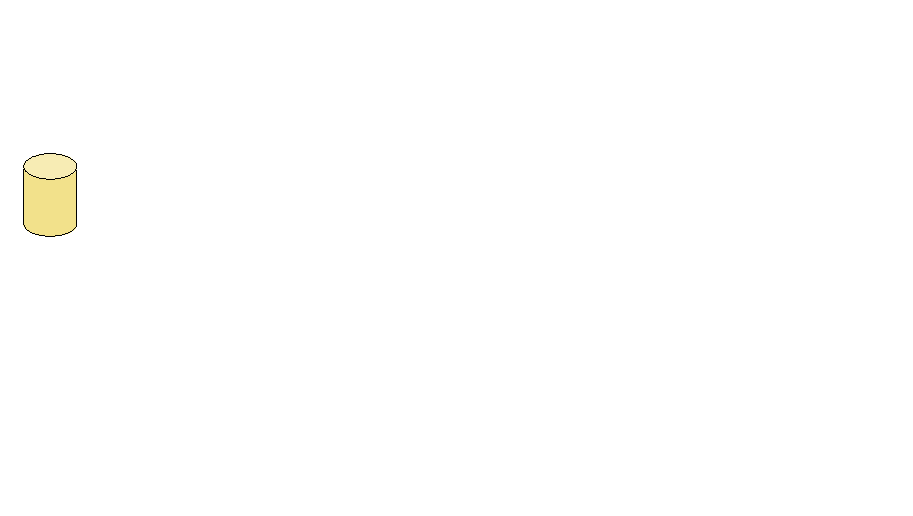
\includegraphics[width=\textwidth]{proposed_architecture.eps}
		\caption{Proposed Architecture}%
		\label{fig:proposed_architecture}
	\end{figure}

	The software architecture will probably be developed in C++, but other
	languages such as Python may also be employed. The following lists the main
	design goals of the proposed architecture:

	\begin{enumerate}

		\item\label{goal:flexibile}

			Be flexible and extendible.

		\item\label{goal:guarantee_trajectory}

			Guarantee collision free trajectories.

	\end{enumerate}

	Goal~\ref{goal:flexibile} may be achieved by adhering to good coding
	practices, whereas Goal~\ref{goal:guarantee_trajectory} is more algorithmic
	in nature. It requires a good understanding and implementation of algorithms
	and methods such as those reported in this literature study.

	One point that may be worth exploring is the generation of an architecture
	that can adapt to different \gls{cdpr} structures. This will require the
	creation of a configuration file format that describes the topology of the
	robot. This is represented as the ``Robot Topology'' database in
	Figure~\ref{fig:proposed_architecture} and may help to further
	Goal~\ref{goal:flexibile}. Furthermore, the steps denoted in
	Figure~\ref{fig:proposed_architecture} should be designed as separate
	modules that adhere to a predetermined interface. This will enable them to
	be interchanged with other modules and algorithms during the progression of
	the thesis.

	With a knowledge of the topology, the architecture will be capable of
	building an internal representation of the robot. Using a type of
	semi-algebraic representation such as those discussed in
	Section~\ref{sec:semi_algebraic_representation_of_bodies} seems to be the
	most promising at present, but other representations may also be
	investigated. A similar approach can be used to model obstacles in the
	world.

	It may be expensive to evaluate the workspace of the robot using methods
	from Section~\ref{sec:continuous_workspace_determination}, but may be worth
	investigating such an approach. Persisting the workspace representation
	could save time in future calculations. The main potential benefit of
	modelling the workspace is that it could potentially limit the total
	configuration space that needs to be searched for a path.

	$\configurationspace$ should ideally be sampled in such a way as to allow
	multiple queries, thereby improving the overall response time of the
	architecture. To this end, $\configurationspace_{\freeregion}$ will be
	represented in a topological graph $\topologicalgraph$ that can be used with
	classical discrete graph search algorithms. Depending on the path planning
	algorithm used, it might be necessary to smooth the calculated path. This is
	currently envisioned as a step after the path has been calculated and may be
	implemented by following methods similar to that described in
	Section~\ref{sec:smoothing_random_paths}.

	The path generated by the architecture should ideally not yet encode any
	timing of the final trajectory. The ``Generate Trajectory'' step of
	Figure~\ref{fig:proposed_architecture} should instead translate the path
	into a time-dependent trajectory. Methods from
	Chapter~\ref{sec:trajectory_generation} may be used in this step. Finally,
	it may be necessary to employ post-processing methods discussed in
	Section~\ref{sec:trajectory_scaling} to meet dynamic requirements of the
	trajectory.


    \printbibliography{}

\end{document}
